% Generated by Sphinx.
\def\sphinxdocclass{report}
\documentclass[a4paper,10pt,english]{sphinxmanual}
\usepackage[utf8]{inputenc}
\DeclareUnicodeCharacter{00A0}{\nobreakspace}
\usepackage{cmap}
\usepackage[T1]{fontenc}
\usepackage{babel}
\usepackage{times}
\usepackage[Bjarne]{fncychap}
\usepackage{longtable}
\usepackage{sphinx}
\usepackage{multirow}


\title{BIP - Bayesian Inference with Python Documentation}
\date{2014-05-27}
\release{0.5.13}
\author{Flávio Codeço Coelho}
\newcommand{\sphinxlogo}{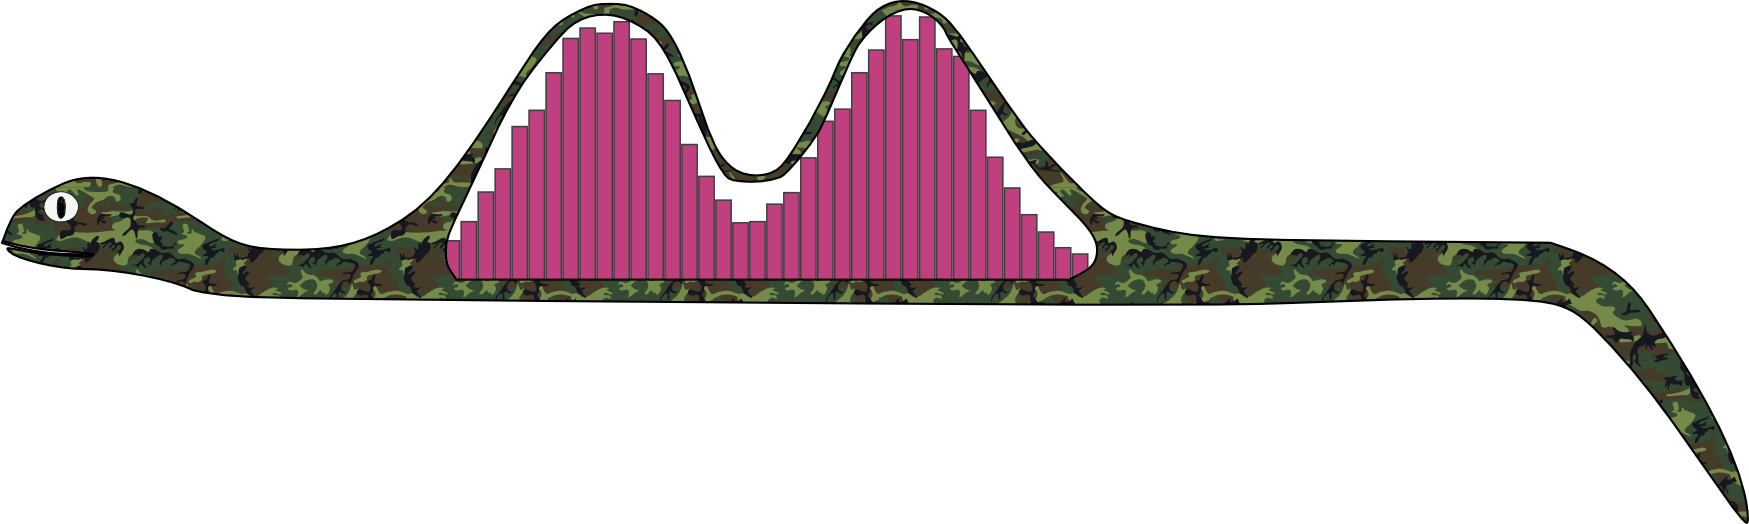
\includegraphics{BIP_large.png}\par}
\renewcommand{\releasename}{Release}
\makeindex

\makeatletter
\def\PYG@reset{\let\PYG@it=\relax \let\PYG@bf=\relax%
    \let\PYG@ul=\relax \let\PYG@tc=\relax%
    \let\PYG@bc=\relax \let\PYG@ff=\relax}
\def\PYG@tok#1{\csname PYG@tok@#1\endcsname}
\def\PYG@toks#1+{\ifx\relax#1\empty\else%
    \PYG@tok{#1}\expandafter\PYG@toks\fi}
\def\PYG@do#1{\PYG@bc{\PYG@tc{\PYG@ul{%
    \PYG@it{\PYG@bf{\PYG@ff{#1}}}}}}}
\def\PYG#1#2{\PYG@reset\PYG@toks#1+\relax+\PYG@do{#2}}

\expandafter\def\csname PYG@tok@gd\endcsname{\def\PYG@tc##1{\textcolor[rgb]{0.63,0.00,0.00}{##1}}}
\expandafter\def\csname PYG@tok@gu\endcsname{\let\PYG@bf=\textbf\def\PYG@tc##1{\textcolor[rgb]{0.50,0.00,0.50}{##1}}}
\expandafter\def\csname PYG@tok@gt\endcsname{\def\PYG@tc##1{\textcolor[rgb]{0.00,0.27,0.87}{##1}}}
\expandafter\def\csname PYG@tok@gs\endcsname{\let\PYG@bf=\textbf}
\expandafter\def\csname PYG@tok@gr\endcsname{\def\PYG@tc##1{\textcolor[rgb]{1.00,0.00,0.00}{##1}}}
\expandafter\def\csname PYG@tok@cm\endcsname{\let\PYG@it=\textit\def\PYG@tc##1{\textcolor[rgb]{0.25,0.50,0.56}{##1}}}
\expandafter\def\csname PYG@tok@vg\endcsname{\def\PYG@tc##1{\textcolor[rgb]{0.73,0.38,0.84}{##1}}}
\expandafter\def\csname PYG@tok@m\endcsname{\def\PYG@tc##1{\textcolor[rgb]{0.13,0.50,0.31}{##1}}}
\expandafter\def\csname PYG@tok@mh\endcsname{\def\PYG@tc##1{\textcolor[rgb]{0.13,0.50,0.31}{##1}}}
\expandafter\def\csname PYG@tok@cs\endcsname{\def\PYG@tc##1{\textcolor[rgb]{0.25,0.50,0.56}{##1}}\def\PYG@bc##1{\setlength{\fboxsep}{0pt}\colorbox[rgb]{1.00,0.94,0.94}{\strut ##1}}}
\expandafter\def\csname PYG@tok@ge\endcsname{\let\PYG@it=\textit}
\expandafter\def\csname PYG@tok@vc\endcsname{\def\PYG@tc##1{\textcolor[rgb]{0.73,0.38,0.84}{##1}}}
\expandafter\def\csname PYG@tok@il\endcsname{\def\PYG@tc##1{\textcolor[rgb]{0.13,0.50,0.31}{##1}}}
\expandafter\def\csname PYG@tok@go\endcsname{\def\PYG@tc##1{\textcolor[rgb]{0.20,0.20,0.20}{##1}}}
\expandafter\def\csname PYG@tok@cp\endcsname{\def\PYG@tc##1{\textcolor[rgb]{0.00,0.44,0.13}{##1}}}
\expandafter\def\csname PYG@tok@gi\endcsname{\def\PYG@tc##1{\textcolor[rgb]{0.00,0.63,0.00}{##1}}}
\expandafter\def\csname PYG@tok@gh\endcsname{\let\PYG@bf=\textbf\def\PYG@tc##1{\textcolor[rgb]{0.00,0.00,0.50}{##1}}}
\expandafter\def\csname PYG@tok@ni\endcsname{\let\PYG@bf=\textbf\def\PYG@tc##1{\textcolor[rgb]{0.84,0.33,0.22}{##1}}}
\expandafter\def\csname PYG@tok@nl\endcsname{\let\PYG@bf=\textbf\def\PYG@tc##1{\textcolor[rgb]{0.00,0.13,0.44}{##1}}}
\expandafter\def\csname PYG@tok@nn\endcsname{\let\PYG@bf=\textbf\def\PYG@tc##1{\textcolor[rgb]{0.05,0.52,0.71}{##1}}}
\expandafter\def\csname PYG@tok@no\endcsname{\def\PYG@tc##1{\textcolor[rgb]{0.38,0.68,0.84}{##1}}}
\expandafter\def\csname PYG@tok@na\endcsname{\def\PYG@tc##1{\textcolor[rgb]{0.25,0.44,0.63}{##1}}}
\expandafter\def\csname PYG@tok@nb\endcsname{\def\PYG@tc##1{\textcolor[rgb]{0.00,0.44,0.13}{##1}}}
\expandafter\def\csname PYG@tok@nc\endcsname{\let\PYG@bf=\textbf\def\PYG@tc##1{\textcolor[rgb]{0.05,0.52,0.71}{##1}}}
\expandafter\def\csname PYG@tok@nd\endcsname{\let\PYG@bf=\textbf\def\PYG@tc##1{\textcolor[rgb]{0.33,0.33,0.33}{##1}}}
\expandafter\def\csname PYG@tok@ne\endcsname{\def\PYG@tc##1{\textcolor[rgb]{0.00,0.44,0.13}{##1}}}
\expandafter\def\csname PYG@tok@nf\endcsname{\def\PYG@tc##1{\textcolor[rgb]{0.02,0.16,0.49}{##1}}}
\expandafter\def\csname PYG@tok@si\endcsname{\let\PYG@it=\textit\def\PYG@tc##1{\textcolor[rgb]{0.44,0.63,0.82}{##1}}}
\expandafter\def\csname PYG@tok@s2\endcsname{\def\PYG@tc##1{\textcolor[rgb]{0.25,0.44,0.63}{##1}}}
\expandafter\def\csname PYG@tok@vi\endcsname{\def\PYG@tc##1{\textcolor[rgb]{0.73,0.38,0.84}{##1}}}
\expandafter\def\csname PYG@tok@nt\endcsname{\let\PYG@bf=\textbf\def\PYG@tc##1{\textcolor[rgb]{0.02,0.16,0.45}{##1}}}
\expandafter\def\csname PYG@tok@nv\endcsname{\def\PYG@tc##1{\textcolor[rgb]{0.73,0.38,0.84}{##1}}}
\expandafter\def\csname PYG@tok@s1\endcsname{\def\PYG@tc##1{\textcolor[rgb]{0.25,0.44,0.63}{##1}}}
\expandafter\def\csname PYG@tok@gp\endcsname{\let\PYG@bf=\textbf\def\PYG@tc##1{\textcolor[rgb]{0.78,0.36,0.04}{##1}}}
\expandafter\def\csname PYG@tok@sh\endcsname{\def\PYG@tc##1{\textcolor[rgb]{0.25,0.44,0.63}{##1}}}
\expandafter\def\csname PYG@tok@ow\endcsname{\let\PYG@bf=\textbf\def\PYG@tc##1{\textcolor[rgb]{0.00,0.44,0.13}{##1}}}
\expandafter\def\csname PYG@tok@sx\endcsname{\def\PYG@tc##1{\textcolor[rgb]{0.78,0.36,0.04}{##1}}}
\expandafter\def\csname PYG@tok@bp\endcsname{\def\PYG@tc##1{\textcolor[rgb]{0.00,0.44,0.13}{##1}}}
\expandafter\def\csname PYG@tok@c1\endcsname{\let\PYG@it=\textit\def\PYG@tc##1{\textcolor[rgb]{0.25,0.50,0.56}{##1}}}
\expandafter\def\csname PYG@tok@kc\endcsname{\let\PYG@bf=\textbf\def\PYG@tc##1{\textcolor[rgb]{0.00,0.44,0.13}{##1}}}
\expandafter\def\csname PYG@tok@c\endcsname{\let\PYG@it=\textit\def\PYG@tc##1{\textcolor[rgb]{0.25,0.50,0.56}{##1}}}
\expandafter\def\csname PYG@tok@mf\endcsname{\def\PYG@tc##1{\textcolor[rgb]{0.13,0.50,0.31}{##1}}}
\expandafter\def\csname PYG@tok@err\endcsname{\def\PYG@bc##1{\setlength{\fboxsep}{0pt}\fcolorbox[rgb]{1.00,0.00,0.00}{1,1,1}{\strut ##1}}}
\expandafter\def\csname PYG@tok@kd\endcsname{\let\PYG@bf=\textbf\def\PYG@tc##1{\textcolor[rgb]{0.00,0.44,0.13}{##1}}}
\expandafter\def\csname PYG@tok@ss\endcsname{\def\PYG@tc##1{\textcolor[rgb]{0.32,0.47,0.09}{##1}}}
\expandafter\def\csname PYG@tok@sr\endcsname{\def\PYG@tc##1{\textcolor[rgb]{0.14,0.33,0.53}{##1}}}
\expandafter\def\csname PYG@tok@mo\endcsname{\def\PYG@tc##1{\textcolor[rgb]{0.13,0.50,0.31}{##1}}}
\expandafter\def\csname PYG@tok@mi\endcsname{\def\PYG@tc##1{\textcolor[rgb]{0.13,0.50,0.31}{##1}}}
\expandafter\def\csname PYG@tok@kn\endcsname{\let\PYG@bf=\textbf\def\PYG@tc##1{\textcolor[rgb]{0.00,0.44,0.13}{##1}}}
\expandafter\def\csname PYG@tok@o\endcsname{\def\PYG@tc##1{\textcolor[rgb]{0.40,0.40,0.40}{##1}}}
\expandafter\def\csname PYG@tok@kr\endcsname{\let\PYG@bf=\textbf\def\PYG@tc##1{\textcolor[rgb]{0.00,0.44,0.13}{##1}}}
\expandafter\def\csname PYG@tok@s\endcsname{\def\PYG@tc##1{\textcolor[rgb]{0.25,0.44,0.63}{##1}}}
\expandafter\def\csname PYG@tok@kp\endcsname{\def\PYG@tc##1{\textcolor[rgb]{0.00,0.44,0.13}{##1}}}
\expandafter\def\csname PYG@tok@w\endcsname{\def\PYG@tc##1{\textcolor[rgb]{0.73,0.73,0.73}{##1}}}
\expandafter\def\csname PYG@tok@kt\endcsname{\def\PYG@tc##1{\textcolor[rgb]{0.56,0.13,0.00}{##1}}}
\expandafter\def\csname PYG@tok@sc\endcsname{\def\PYG@tc##1{\textcolor[rgb]{0.25,0.44,0.63}{##1}}}
\expandafter\def\csname PYG@tok@sb\endcsname{\def\PYG@tc##1{\textcolor[rgb]{0.25,0.44,0.63}{##1}}}
\expandafter\def\csname PYG@tok@k\endcsname{\let\PYG@bf=\textbf\def\PYG@tc##1{\textcolor[rgb]{0.00,0.44,0.13}{##1}}}
\expandafter\def\csname PYG@tok@se\endcsname{\let\PYG@bf=\textbf\def\PYG@tc##1{\textcolor[rgb]{0.25,0.44,0.63}{##1}}}
\expandafter\def\csname PYG@tok@sd\endcsname{\let\PYG@it=\textit\def\PYG@tc##1{\textcolor[rgb]{0.25,0.44,0.63}{##1}}}

\def\PYGZbs{\char`\\}
\def\PYGZus{\char`\_}
\def\PYGZob{\char`\{}
\def\PYGZcb{\char`\}}
\def\PYGZca{\char`\^}
\def\PYGZam{\char`\&}
\def\PYGZlt{\char`\<}
\def\PYGZgt{\char`\>}
\def\PYGZsh{\char`\#}
\def\PYGZpc{\char`\%}
\def\PYGZdl{\char`\$}
\def\PYGZhy{\char`\-}
\def\PYGZsq{\char`\'}
\def\PYGZdq{\char`\"}
\def\PYGZti{\char`\~}
% for compatibility with earlier versions
\def\PYGZat{@}
\def\PYGZlb{[}
\def\PYGZrb{]}
\makeatother

\begin{document}

\maketitle
\tableofcontents
\phantomsection\label{index::doc}


This documentation corresponds to version 0.5.13.


\chapter{Contents}
\label{index:contents}\label{index:welcome-to-bip-bayesian-inference-with-python-s-documentation}

\section{Overview}
\label{overview:overview}\label{overview::doc}
The Bip Package is a collection of useful classes for basic Bayesian inference. Currently, its main goal is to be a tool for learning and exploration of Bayesian probabilistic calculations.

Currently it also includes subpackages for stochastic simulation tools which are not strictly related to Bayesian inference, but are currently being developed within BIP. One such package is the BIP.SDE which contains a parallelized solver for stochastic differential equations, an implementation of the Gillespie direct algorithm.

The Subpackage Bayes also offers a tool for parameter estimation of Deterministic and Stochastic Dynamical Models. This tool will be fully described briefly in a scientific paper currently submitted for publication.


\section{Parameter Estimation in Dynamic Models}
\label{paramest:parameter-estimation-in-dynamic-models}\label{paramest::doc}
A growing theme in mathematical modeling is uncertainty analysis. The Melding Module provides a Bayesian framework to analyze uncertainty in mathematical models. It includes tools that allow modellers to integrate Prior information about the model's parameters and variables into the model, in order to explore the full uncertainty associated with a model.

This framework is inspired on the original Bayesian Melding paper by Poole and Raftery \footnote{
Poole, D., \& Raftery, A. E. (2000). Inference for Deterministic Simulation Models: The Bayesian Melding Approach. Journal of the American Statistical Association, 95(452), 1244-1255. doi:10.2307/2669764
}, but extended to handle dynamical systems and different posterior sampling mechanisms, i.e., the user has the choice to use Sampling Importance resampling, Approximate Bayesian computations or MCMC. A deeper description of the methodology implemented in this package is available as published research paper \footnote{
Coelho FC, Codeço CT, Gomes MGM (2011) A Bayesian Framework for Parameter Estimation in Dynamical Models. PLoS ONE 6(5): e19616. doi:10.1371/journal.pone.0019616
}. This paper also contains a more extensive example of parameter estimation. If you intend to use this package for a scientific publication, you should cite this paper \footnotemark[1].

Once a model is thus parameterized, we can simulate the model, with full uncertainty representation and also fit the model to available data to reduce that uncertaity. Markov chain Monte Carlo algorithms are at the core of the framework, which requires a large number of simulations of the models in order to explore parameter space.


\subsection{Single Session Retrospective estimation}
\label{paramest:single-session-retrospective-estimation}
Frequently, we have a complete time series corresponding to one or more state variables of our dynamic model. In such cases it may be interesting to use this information, to estimate the parameter values which maximize the fit of our model to the data. Below are examples of such inference situations.


\subsubsection{Example Usage}
\label{paramest:example-usage}
This first example includes a simple ODE (an SIR epidemic model) model which is fitted against simulated data to which noise is added:

\begin{Verbatim}[commandchars=\\\{\}]
\PYG{c}{\PYGZsh{}\PYGZhy{}*\PYGZhy{} coding: utf\PYGZhy{}8 \PYGZhy{}*\PYGZhy{}}
\PYG{l+s+sd}{\PYGZdq{}\PYGZdq{}\PYGZdq{}}
\PYG{l+s+sd}{Parameter estimation and series forcasting based on simulated data with moving window.}
\PYG{l+s+sd}{Deterministic model}
\PYG{l+s+sd}{\PYGZdq{}\PYGZdq{}\PYGZdq{}}
\PYG{c}{\PYGZsh{}}
\PYG{c}{\PYGZsh{} Copyright 2009\PYGZhy{} by Flávio Codeço Coelho}
\PYG{c}{\PYGZsh{} License gpl v3}
\PYG{c}{\PYGZsh{}}
\PYG{k+kn}{from} \PYG{n+nn}{BIP.Bayes.Melding} \PYG{k+kn}{import} \PYG{n}{FitModel}
\PYG{k+kn}{from} \PYG{n+nn}{scipy.integrate} \PYG{k+kn}{import} \PYG{n}{odeint}
\PYG{k+kn}{import} \PYG{n+nn}{scipy.stats} \PYG{k+kn}{as} \PYG{n+nn}{st}
\PYG{k+kn}{import} \PYG{n+nn}{numpy} \PYG{k+kn}{as} \PYG{n+nn}{np}

\PYG{n}{beta} \PYG{o}{=} \PYG{l+m+mi}{1} \PYG{c}{\PYGZsh{}Transmission coefficient}
\PYG{n}{tau} \PYG{o}{=} \PYG{o}{.}\PYG{l+m+mi}{2} \PYG{c}{\PYGZsh{}infectious period. FIXED}
\PYG{n}{tf} \PYG{o}{=} \PYG{l+m+mi}{36}
\PYG{n}{y0} \PYG{o}{=} \PYG{p}{[}\PYG{o}{.}\PYG{l+m+mi}{999}\PYG{p}{,}\PYG{l+m+mf}{0.001}\PYG{p}{,}\PYG{l+m+mf}{0.0}\PYG{p}{]}
\PYG{k}{def} \PYG{n+nf}{model}\PYG{p}{(}\PYG{n}{theta}\PYG{p}{)}\PYG{p}{:}
    \PYG{n}{beta} \PYG{o}{=} \PYG{n}{theta}\PYG{p}{[}\PYG{l+m+mi}{0}\PYG{p}{]}
    \PYG{k}{def} \PYG{n+nf}{sir}\PYG{p}{(}\PYG{n}{y}\PYG{p}{,}\PYG{n}{t}\PYG{p}{)}\PYG{p}{:}
        \PYG{l+s+sd}{\PYGZsq{}\PYGZsq{}\PYGZsq{}ODE model\PYGZsq{}\PYGZsq{}\PYGZsq{}}
        \PYG{n}{S}\PYG{p}{,}\PYG{n}{I}\PYG{p}{,}\PYG{n}{R} \PYG{o}{=} \PYG{n}{y}
        \PYG{k}{return}  \PYG{p}{[}\PYG{o}{\PYGZhy{}}\PYG{n}{beta}\PYG{o}{*}\PYG{n}{I}\PYG{o}{*}\PYG{n}{S}\PYG{p}{,} \PYG{c}{\PYGZsh{}dS/dt}
                \PYG{n}{beta}\PYG{o}{*}\PYG{n}{I}\PYG{o}{*}\PYG{n}{S} \PYG{o}{\PYGZhy{}} \PYG{n}{tau}\PYG{o}{*}\PYG{n}{I}\PYG{p}{,} \PYG{c}{\PYGZsh{}dI/dt}
                \PYG{n}{tau}\PYG{o}{*}\PYG{n}{I}\PYG{p}{]} \PYG{c}{\PYGZsh{}dR/dt}
    \PYG{n}{y} \PYG{o}{=} \PYG{n}{odeint}\PYG{p}{(}\PYG{n}{sir}\PYG{p}{,}\PYG{n}{inits}\PYG{p}{,}\PYG{n}{np}\PYG{o}{.}\PYG{n}{arange}\PYG{p}{(}\PYG{l+m+mi}{0}\PYG{p}{,}\PYG{n}{tf}\PYG{p}{,}\PYG{l+m+mi}{1}\PYG{p}{)}\PYG{p}{)}
    \PYG{k}{return} \PYG{n}{y}
    
\PYG{n}{F} \PYG{o}{=} \PYG{n}{FitModel}\PYG{p}{(}\PYG{l+m+mi}{500}\PYG{p}{,} \PYG{n}{model}\PYG{p}{,}\PYG{n}{y0}\PYG{p}{,}\PYG{n}{tf}\PYG{p}{,}\PYG{p}{[}\PYG{l+s}{\PYGZsq{}}\PYG{l+s}{beta}\PYG{l+s}{\PYGZsq{}}\PYG{p}{]}\PYG{p}{,}\PYG{p}{[}\PYG{l+s}{\PYGZsq{}}\PYG{l+s}{S}\PYG{l+s}{\PYGZsq{}}\PYG{p}{,}\PYG{l+s}{\PYGZsq{}}\PYG{l+s}{I}\PYG{l+s}{\PYGZsq{}}\PYG{p}{,}\PYG{l+s}{\PYGZsq{}}\PYG{l+s}{R}\PYG{l+s}{\PYGZsq{}}\PYG{p}{]}\PYG{p}{,}
            \PYG{n}{wl}\PYG{o}{=}\PYG{l+m+mi}{36}\PYG{p}{,}\PYG{n}{nw}\PYG{o}{=}\PYG{l+m+mi}{1}\PYG{p}{,}\PYG{n}{verbose}\PYG{o}{=}\PYG{l+m+mi}{0}\PYG{p}{,}\PYG{n}{burnin}\PYG{o}{=}\PYG{l+m+mi}{100}\PYG{p}{)}
\PYG{n}{F}\PYG{o}{.}\PYG{n}{set\PYGZus{}priors}\PYG{p}{(}\PYG{n}{tdists}\PYG{o}{=}\PYG{p}{[}\PYG{n}{st}\PYG{o}{.}\PYG{n}{norm}\PYG{p}{]}\PYG{p}{,}\PYG{n}{tpars}\PYG{o}{=}\PYG{p}{[}\PYG{p}{(}\PYG{l+m+mf}{1.1}\PYG{p}{,}\PYG{o}{.}\PYG{l+m+mi}{2}\PYG{p}{)}\PYG{p}{]}\PYG{p}{,}\PYG{n}{tlims}\PYG{o}{=}\PYG{p}{[}\PYG{p}{(}\PYG{l+m+mf}{0.5}\PYG{p}{,}\PYG{l+m+mf}{1.5}\PYG{p}{)}\PYG{p}{]}\PYG{p}{,}
    \PYG{n}{pdists}\PYG{o}{=}\PYG{p}{[}\PYG{n}{st}\PYG{o}{.}\PYG{n}{uniform}\PYG{p}{]}\PYG{o}{*}\PYG{l+m+mi}{3}\PYG{p}{,}\PYG{n}{ppars}\PYG{o}{=}\PYG{p}{[}\PYG{p}{(}\PYG{l+m+mi}{0}\PYG{p}{,}\PYG{o}{.}\PYG{l+m+mi}{1}\PYG{p}{)}\PYG{p}{,}\PYG{p}{(}\PYG{l+m+mi}{0}\PYG{p}{,}\PYG{o}{.}\PYG{l+m+mi}{1}\PYG{p}{)}\PYG{p}{,}\PYG{p}{(}\PYG{o}{.}\PYG{l+m+mi}{8}\PYG{p}{,}\PYG{o}{.}\PYG{l+m+mi}{2}\PYG{p}{)}\PYG{p}{]}\PYG{p}{,}\PYG{n}{plims}\PYG{o}{=}\PYG{p}{[}\PYG{p}{(}\PYG{l+m+mi}{0}\PYG{p}{,}\PYG{l+m+mi}{1}\PYG{p}{)}\PYG{p}{]}\PYG{o}{*}\PYG{l+m+mi}{3}\PYG{p}{)}
\PYG{n}{d} \PYG{o}{=} \PYG{n}{model}\PYG{p}{(}\PYG{p}{[}\PYG{l+m+mf}{1.0}\PYG{p}{]}\PYG{p}{)} \PYG{c}{\PYGZsh{}simulate some data}
\PYG{n}{noise} \PYG{o}{=} \PYG{n}{st}\PYG{o}{.}\PYG{n}{norm}\PYG{p}{(}\PYG{l+m+mi}{0}\PYG{p}{,}\PYG{l+m+mf}{0.01}\PYG{p}{)}\PYG{o}{.}\PYG{n}{rvs}\PYG{p}{(}\PYG{l+m+mi}{36}\PYG{p}{)}
\PYG{n}{dt} \PYG{o}{=} \PYG{p}{\PYGZob{}}\PYG{l+s}{\PYGZsq{}}\PYG{l+s}{I}\PYG{l+s}{\PYGZsq{}}\PYG{p}{:}\PYG{n}{d}\PYG{p}{[}\PYG{p}{:}\PYG{p}{,}\PYG{l+m+mi}{1}\PYG{p}{]}\PYG{o}{+}\PYG{n}{noise}\PYG{p}{\PYGZcb{}} \PYG{c}{\PYGZsh{} add noise}
\PYG{n}{F}\PYG{o}{.}\PYG{n}{run}\PYG{p}{(}\PYG{n}{dt}\PYG{p}{,}\PYG{l+s}{\PYGZsq{}}\PYG{l+s}{MCMC}\PYG{l+s}{\PYGZsq{}}\PYG{p}{,}\PYG{n}{likvar}\PYG{o}{=}\PYG{l+m+mf}{1e\PYGZhy{}5}\PYG{p}{,}\PYG{n}{pool}\PYG{o}{=}\PYG{n+nb+bp}{True}\PYG{p}{,}\PYG{n}{monitor}\PYG{o}{=}\PYG{p}{[}\PYG{p}{]}\PYG{p}{)}
\PYG{c}{\PYGZsh{}==Uncomment the line below to see plots of the results}
\PYG{n}{F}\PYG{o}{.}\PYG{n}{plot\PYGZus{}results}\PYG{p}{(}\PYG{p}{)}
\end{Verbatim}

The code above starts by defining the models parameters and initial conditions, and a function which takes in the parameters runs the model and returns the output.

After that, we Instantiate our fitting Object:

\begin{Verbatim}[commandchars=\\\{\}]
\PYG{n}{F} \PYG{o}{=} \PYG{n}{FitModel}\PYG{p}{(}\PYG{l+m+mi}{300}\PYG{p}{,}\PYG{n}{model}\PYG{p}{,}\PYG{n}{y0}\PYG{p}{,}\PYG{n}{tf}\PYG{p}{,}\PYG{p}{[}\PYG{l+s}{\PYGZsq{}}\PYG{l+s}{beta}\PYG{l+s}{\PYGZsq{}}\PYG{p}{]}\PYG{p}{,}\PYG{p}{[}\PYG{l+s}{\PYGZsq{}}\PYG{l+s}{S}\PYG{l+s}{\PYGZsq{}}\PYG{p}{,}\PYG{l+s}{\PYGZsq{}}\PYG{l+s}{I}\PYG{l+s}{\PYGZsq{}}\PYG{p}{,}\PYG{l+s}{\PYGZsq{}}\PYG{l+s}{R}\PYG{l+s}{\PYGZsq{}}\PYG{p}{]}\PYG{p}{,}
            \PYG{n}{wl}\PYG{o}{=}\PYG{l+m+mi}{36}\PYG{p}{,}\PYG{n}{nw}\PYG{o}{=}\PYG{l+m+mi}{1}\PYG{p}{,}\PYG{n}{verbose}\PYG{o}{=}\PYG{n+nb+bp}{False}\PYG{p}{,}\PYG{n}{burnin}\PYG{o}{=}\PYG{l+m+mi}{100}\PYG{p}{)}
\end{Verbatim}

Here we have to pass a few arguments: the first (\code{K=300}) is the number of samples we will take from the joint prior distribution of the parameters to run the inference. The second one (\code{model}) is the callable(function) which corresponds to the model you want to fit to data. Then you have the initial condition vector(\code{inits=y0}), the list of parameter names (\code{thetanames = {[}'beta'{]}}), the list of variable names (\code{phinames={[}'S','I','R'{]}}), inference window length (\code{wl=36}), number of juxtaposed windows (\code{nw=1}), verbosity flag (\code{verbose=False}) and finally the number of burnin samples (\code{burnin=1000}), which is only needed for if the inference method chosen is \code{MCMC}.

One should always have \code{verbose=True} on a first fitting run of a model or if the simulations seems to be taking longer than expected. When \code{verbose} is true, printed and graphical is generated regarding the behavior of fitting, which can be useful to fine tune its parameters.

The next line of code also carries a lot of relevant information about the inference: the specification of the prior distributions. By now you must have noticed that not all parameters included in the model need to be included in the analysis. any number of them except for one can be set constant, which is what happens with the parameter \code{tau} in this example:

\begin{Verbatim}[commandchars=\\\{\}]
\PYG{n}{F}\PYG{o}{.}\PYG{n}{set\PYGZus{}priors}\PYG{p}{(}\PYG{n}{tdists}\PYG{o}{=}\PYG{p}{[}\PYG{n}{st}\PYG{o}{.}\PYG{n}{norm}\PYG{p}{]}\PYG{p}{,}\PYG{n}{tpars}\PYG{o}{=}\PYG{p}{[}\PYG{p}{(}\PYG{l+m+mf}{1.1}\PYG{p}{,}\PYG{o}{.}\PYG{l+m+mi}{2}\PYG{p}{)}\PYG{p}{]}\PYG{p}{,}\PYG{n}{tlims}\PYG{o}{=}\PYG{p}{[}\PYG{p}{(}\PYG{l+m+mf}{0.5}\PYG{p}{,}\PYG{l+m+mf}{1.5}\PYG{p}{)}\PYG{p}{]}\PYG{p}{,}
    \PYG{n}{pdists}\PYG{o}{=}\PYG{p}{[}\PYG{n}{st}\PYG{o}{.}\PYG{n}{uniform}\PYG{p}{]}\PYG{o}{*}\PYG{l+m+mi}{3}\PYG{p}{,}\PYG{n}{ppars}\PYG{o}{=}\PYG{p}{[}\PYG{p}{(}\PYG{l+m+mi}{0}\PYG{p}{,}\PYG{o}{.}\PYG{l+m+mi}{1}\PYG{p}{)}\PYG{p}{,}\PYG{p}{(}\PYG{l+m+mi}{0}\PYG{p}{,}\PYG{o}{.}\PYG{l+m+mi}{1}\PYG{p}{)}\PYG{p}{,}\PYG{p}{(}\PYG{o}{.}\PYG{l+m+mi}{8}\PYG{p}{,}\PYG{o}{.}\PYG{l+m+mi}{2}\PYG{p}{)}\PYG{p}{]}\PYG{p}{,}\PYG{n}{plims}\PYG{o}{=}\PYG{p}{[}\PYG{p}{(}\PYG{l+m+mi}{0}\PYG{p}{,}\PYG{l+m+mi}{1}\PYG{p}{)}\PYG{p}{]}\PYG{o}{*}\PYG{l+m+mi}{3}\PYG{p}{)}
\end{Verbatim}

here we set the prior distributions for the theta (the model's parameters) and phi (the model's variables). \code{tdists}, \code{tpars} and \code{tlims} are theta's distributions, parameters, and ranges. For example here we use a Normal distribution (\code{st.norm}) for \code{beta}, with mean and standard deviation equal to 1.1 and .2, respectively. we also set the range of \code{beta} to be from 0.5 to 1.5. We do the same for phi.

The remaining lines just generate some simulated data to fit the model with, run the inference and plot the results which should include plots like this:
\begin{figure}[htbp]
\centering
\capstart

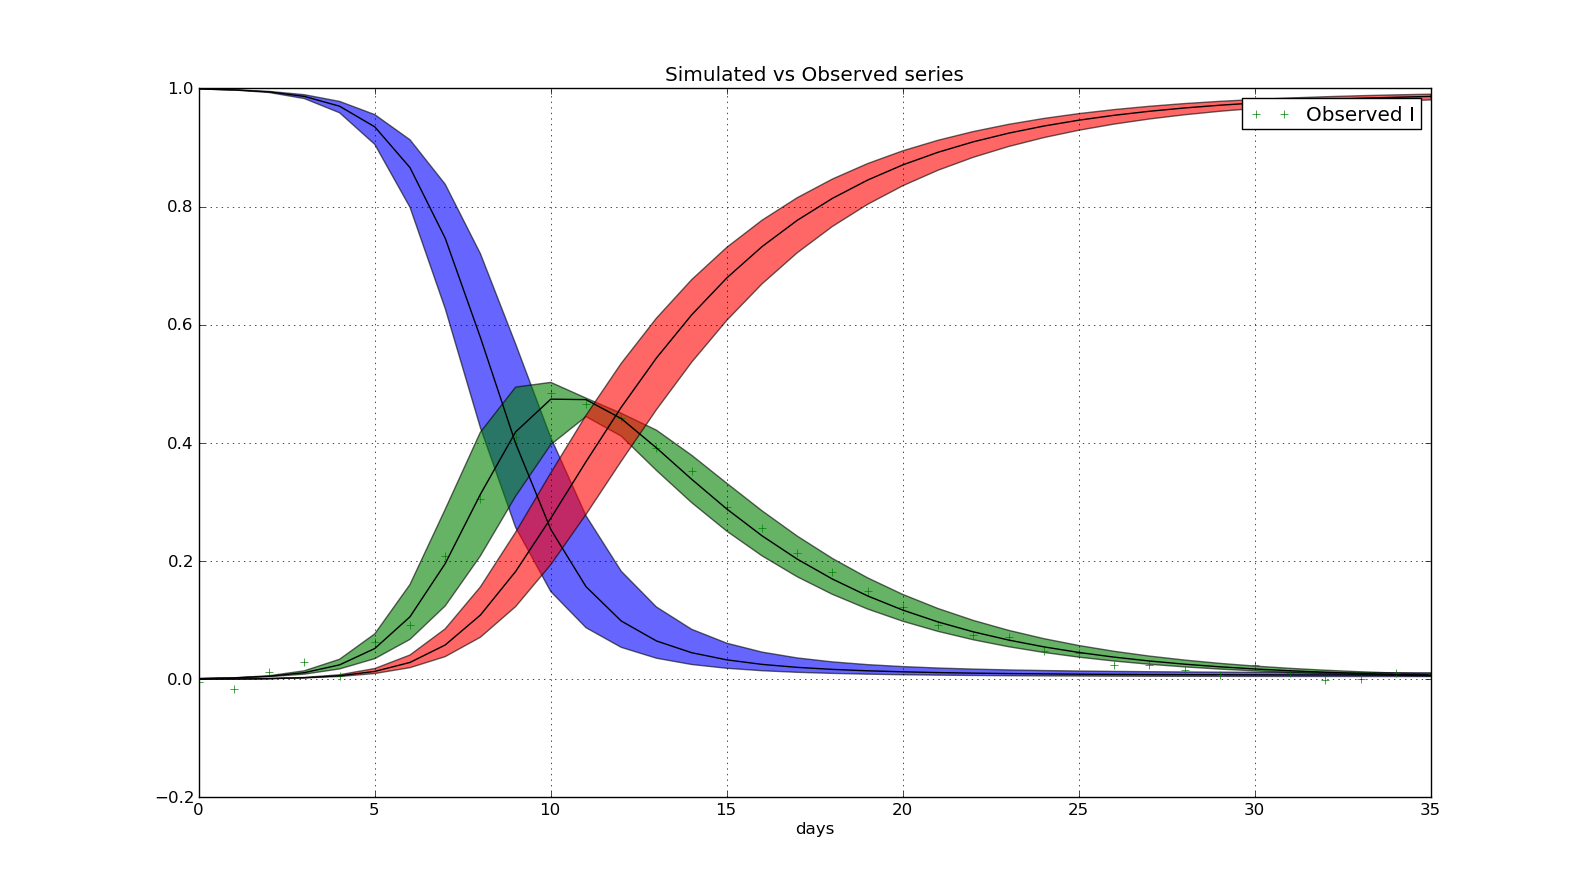
\includegraphics[width=15cm]{fit_series.png}
\caption{Series posterior distributions. Colored areas represent 95\% credible intervals.}\end{figure}
\begin{figure}[htbp]
\centering
\capstart

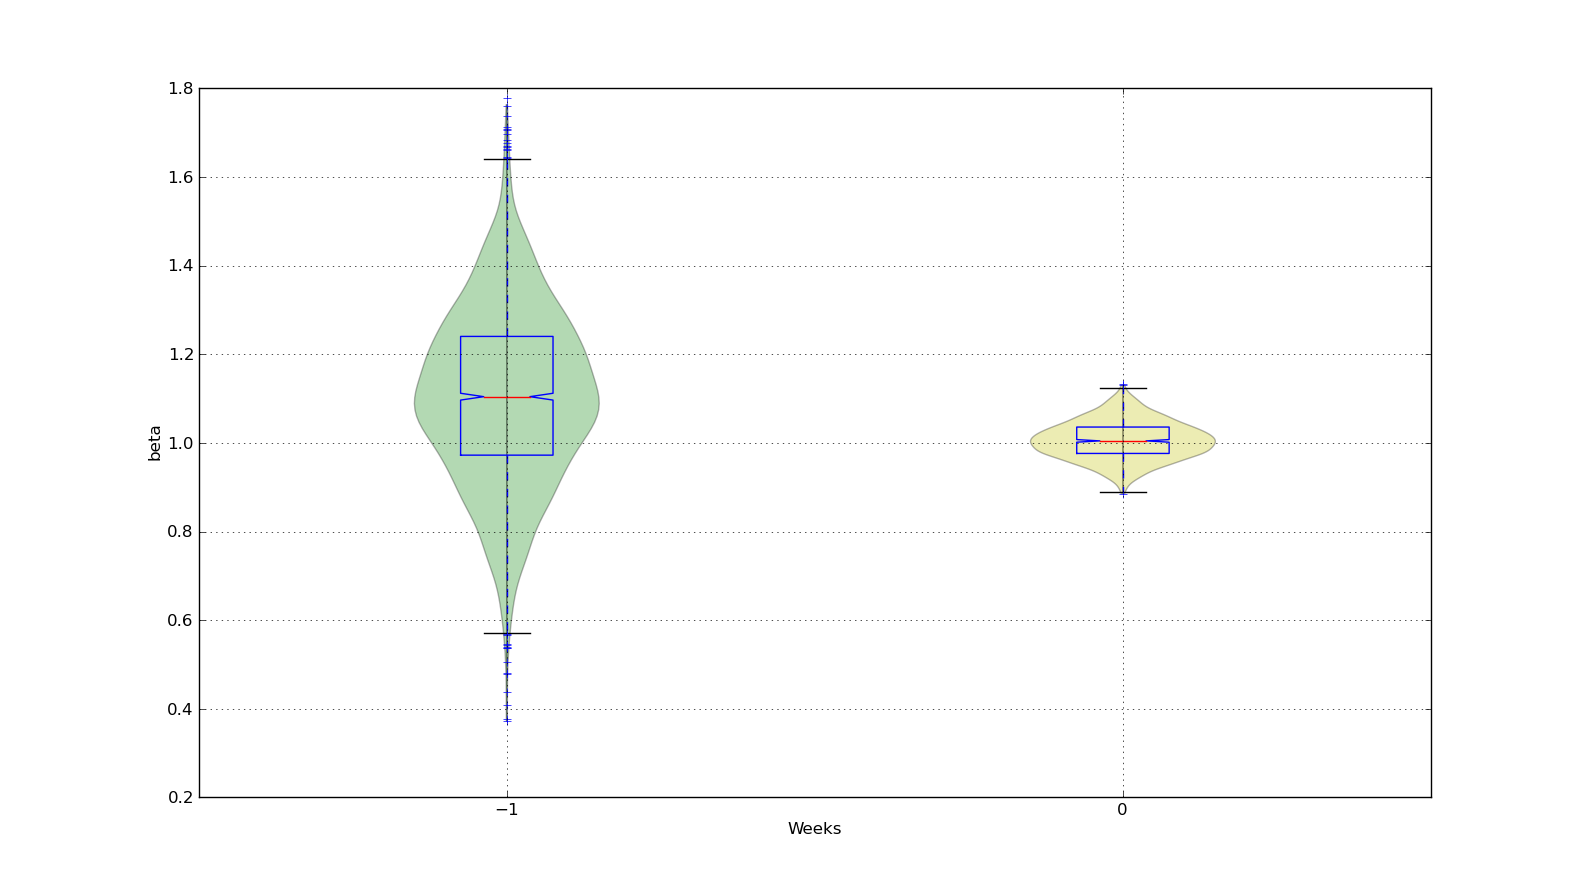
\includegraphics[width=15cm]{fit_par.png}
\caption{Parameters prior and posterior distributions.}\end{figure}

One important argument in the run call, is the likvar, Which is the initial value for the likelihood variance. Try to increase its value if the acceptance ratio of the markov chain is too llow. Ideal levels for the acceptance ratio should be between 0.3 and 0.5.

The code for the above example can be found in the examples directory of the BIP distribution as \code{deterministic.py}


\subsubsection{Stochastic Model Example}
\label{paramest:stochastic-model-example}
This example fits a stochastic model to simulated data. It uses the {\hyperref[sde:sde]{\emph{SDE}}} package of BIP:

\begin{Verbatim}[commandchars=\\\{\}]
\PYG{c}{\PYGZsh{}\PYGZhy{}*\PYGZhy{} coding:utf\PYGZhy{}8 \PYGZhy{}*\PYGZhy{}}
\PYG{l+s+sd}{\PYGZdq{}\PYGZdq{}\PYGZdq{}}
\PYG{l+s+sd}{Parameter estimation and series forcasting based on simulated data with moving window.}
\PYG{l+s+sd}{Stochastic model}
\PYG{l+s+sd}{\PYGZdq{}\PYGZdq{}\PYGZdq{}}
\PYG{c}{\PYGZsh{}}
\PYG{c}{\PYGZsh{} Copyright 2009\PYGZhy{} by Flávio Codeço Coelho}
\PYG{c}{\PYGZsh{} License gpl v3}
\PYG{c}{\PYGZsh{}}
\PYG{k+kn}{from} \PYG{n+nn}{BIP.SDE.gillespie} \PYG{k+kn}{import} \PYG{n}{Model}
\PYG{k+kn}{from} \PYG{n+nn}{BIP.Bayes.Melding} \PYG{k+kn}{import} \PYG{n}{FitModel}
\PYG{k+kn}{import} \PYG{n+nn}{numpy} \PYG{k+kn}{as} \PYG{n+nn}{np}
\PYG{k+kn}{from} \PYG{n+nn}{scipy} \PYG{k+kn}{import} \PYG{n}{stats} \PYG{k}{as} \PYG{n}{st}


\PYG{n}{mu} \PYG{o}{=} \PYG{l+m+mf}{0.0} \PYG{c}{\PYGZsh{}birth and death rate.FIXED}
\PYG{n}{beta} \PYG{o}{=} \PYG{l+m+mf}{0.00058} \PYG{c}{\PYGZsh{}Transmission rate}
\PYG{n}{eta} \PYG{o}{=} \PYG{o}{.}\PYG{l+m+mi}{5} \PYG{c}{\PYGZsh{}infectivity of asymptomatic infections relative to clinical ones. FIXED}
\PYG{n}{epsilon} \PYG{o}{=} \PYG{o}{.}\PYG{l+m+mi}{1} \PYG{c}{\PYGZsh{}latency period }
\PYG{n}{alpha} \PYG{o}{=} \PYG{o}{.}\PYG{l+m+mi}{2} \PYG{c}{\PYGZsh{}Probability of developing clinical influenza symptoms}
\PYG{n}{sigma} \PYG{o}{=} \PYG{o}{.}\PYG{l+m+mi}{5} \PYG{c}{\PYGZsh{}reduced risk of re\PYGZhy{}infection after recovery}
\PYG{n}{tau} \PYG{o}{=} \PYG{o}{.}\PYG{l+m+mo}{01} \PYG{c}{\PYGZsh{}infectious period. FIXED}
\PYG{c}{\PYGZsh{} Initial conditions}
\PYG{k}{global} \PYG{n}{inits}\PYG{p}{,}\PYG{n}{tf}
\PYG{n}{tf}\PYG{o}{=} \PYG{l+m+mi}{140}
\PYG{n}{inits} \PYG{o}{=} \PYG{p}{[}\PYG{l+m+mi}{490}\PYG{p}{,}\PYG{l+m+mi}{0}\PYG{p}{,}\PYG{l+m+mi}{10}\PYG{p}{,}\PYG{l+m+mi}{0}\PYG{p}{,}\PYG{l+m+mi}{0}\PYG{p}{]}
\PYG{n}{pars} \PYG{o}{=} \PYG{p}{[}\PYG{n}{beta}\PYG{p}{,}\PYG{n}{alpha}\PYG{p}{,}\PYG{n}{sigma}\PYG{p}{]}


\PYG{c}{\PYGZsh{} propensity functions}
\PYG{k}{def} \PYG{n+nf}{f1}\PYG{p}{(}\PYG{n}{r}\PYG{p}{,}\PYG{n}{inits}\PYG{p}{)}\PYG{p}{:}\PYG{k}{return} \PYG{n}{r}\PYG{p}{[}\PYG{l+m+mi}{0}\PYG{p}{]}\PYG{o}{*}\PYG{n}{inits}\PYG{p}{[}\PYG{l+m+mi}{0}\PYG{p}{]}\PYG{o}{*}\PYG{p}{(}\PYG{n}{inits}\PYG{p}{[}\PYG{l+m+mi}{2}\PYG{p}{]}\PYG{o}{+}\PYG{n}{inits}\PYG{p}{[}\PYG{l+m+mi}{3}\PYG{p}{]}\PYG{p}{)}\PYG{c}{\PYGZsh{}S\PYGZhy{}\PYGZgt{}E}
\PYG{k}{def} \PYG{n+nf}{f2}\PYG{p}{(}\PYG{n}{r}\PYG{p}{,}\PYG{n}{inits}\PYG{p}{)}\PYG{p}{:}\PYG{k}{return} \PYG{n}{r}\PYG{p}{[}\PYG{l+m+mi}{1}\PYG{p}{]}\PYG{o}{*}\PYG{n}{inits}\PYG{p}{[}\PYG{l+m+mi}{1}\PYG{p}{]}\PYG{c}{\PYGZsh{}E\PYGZhy{}\PYGZgt{}I}
\PYG{k}{def} \PYG{n+nf}{f3}\PYG{p}{(}\PYG{n}{r}\PYG{p}{,}\PYG{n}{inits}\PYG{p}{)}\PYG{p}{:}\PYG{k}{return} \PYG{n}{r}\PYG{p}{[}\PYG{l+m+mi}{3}\PYG{p}{]}\PYG{o}{*}\PYG{n}{inits}\PYG{p}{[}\PYG{l+m+mi}{2}\PYG{p}{]}\PYG{c}{\PYGZsh{}I\PYGZhy{}\PYGZgt{}R}
\PYG{k}{def} \PYG{n+nf}{f4}\PYG{p}{(}\PYG{n}{r}\PYG{p}{,}\PYG{n}{inits}\PYG{p}{)}\PYG{p}{:}\PYG{k}{return} \PYG{n}{r}\PYG{p}{[}\PYG{l+m+mi}{2}\PYG{p}{]}\PYG{o}{*}\PYG{n}{inits}\PYG{p}{[}\PYG{l+m+mi}{1}\PYG{p}{]}\PYG{c}{\PYGZsh{}E\PYGZhy{}\PYGZgt{}A}
\PYG{k}{def} \PYG{n+nf}{f5}\PYG{p}{(}\PYG{n}{r}\PYG{p}{,}\PYG{n}{inits}\PYG{p}{)}\PYG{p}{:}\PYG{k}{return} \PYG{n}{r}\PYG{p}{[}\PYG{l+m+mi}{4}\PYG{p}{]}\PYG{o}{*}\PYG{n}{inits}\PYG{p}{[}\PYG{l+m+mi}{3}\PYG{p}{]}\PYG{c}{\PYGZsh{}A\PYGZhy{}\PYGZgt{}R}

\PYG{k}{def} \PYG{n+nf}{runModel}\PYG{p}{(}\PYG{n}{theta}\PYG{p}{)}\PYG{p}{:}
    \PYG{k}{global} \PYG{n}{tf}\PYG{p}{,}\PYG{n}{inits}
    \PYG{n}{step} \PYG{o}{=} \PYG{l+m+mi}{1}
    \PYG{c}{\PYGZsh{}setting parameters}
    \PYG{n}{beta}\PYG{p}{,}\PYG{n}{alpha}\PYG{p}{,}\PYG{n}{sigma} \PYG{o}{=} \PYG{n}{theta}\PYG{p}{[}\PYG{p}{:}\PYG{l+m+mi}{3}\PYG{p}{]}
    \PYG{n}{vnames} \PYG{o}{=} \PYG{p}{[}\PYG{l+s}{\PYGZsq{}}\PYG{l+s}{S}\PYG{l+s}{\PYGZsq{}}\PYG{p}{,}\PYG{l+s}{\PYGZsq{}}\PYG{l+s}{E}\PYG{l+s}{\PYGZsq{}}\PYG{p}{,}\PYG{l+s}{\PYGZsq{}}\PYG{l+s}{I}\PYG{l+s}{\PYGZsq{}}\PYG{p}{,}\PYG{l+s}{\PYGZsq{}}\PYG{l+s}{A}\PYG{l+s}{\PYGZsq{}}\PYG{p}{,}\PYG{l+s}{\PYGZsq{}}\PYG{l+s}{R}\PYG{l+s}{\PYGZsq{}}\PYG{p}{]}
    \PYG{c}{\PYGZsh{}rates: b,ki,ka,ri,ra}
    \PYG{c}{\PYGZsh{}r = (0.001, 0.1, 0.1, 0.01, 0.01)}
    \PYG{n}{r} \PYG{o}{=} \PYG{p}{(}\PYG{n}{beta}\PYG{p}{,} \PYG{n}{alpha}\PYG{o}{*}\PYG{n}{epsilon}\PYG{p}{,} \PYG{p}{(}\PYG{l+m+mi}{1}\PYG{o}{\PYGZhy{}}\PYG{n}{alpha}\PYG{p}{)}\PYG{o}{*}\PYG{n}{epsilon}\PYG{p}{,} \PYG{n}{tau}\PYG{p}{,} \PYG{n}{tau}\PYG{p}{)}
    \PYG{c}{\PYGZsh{}print r,inits}
    \PYG{c}{\PYGZsh{} propensity functions}
    \PYG{n}{propf} \PYG{o}{=} \PYG{p}{(}\PYG{n}{f1}\PYG{p}{,}\PYG{n}{f2}\PYG{p}{,}\PYG{n}{f3}\PYG{p}{,}\PYG{n}{f4}\PYG{p}{,}\PYG{n}{f5}\PYG{p}{)}

    \PYG{n}{tmat} \PYG{o}{=} \PYG{n}{np}\PYG{o}{.}\PYG{n}{array}\PYG{p}{(}\PYG{p}{[}\PYG{p}{[}\PYG{o}{\PYGZhy{}}\PYG{l+m+mi}{1}\PYG{p}{,} \PYG{l+m+mi}{0}\PYG{p}{,} \PYG{l+m+mi}{0}\PYG{p}{,} \PYG{l+m+mi}{0}\PYG{p}{,} \PYG{l+m+mi}{0}\PYG{p}{]}\PYG{p}{,}
                  \PYG{p}{[} \PYG{l+m+mi}{1}\PYG{p}{,}\PYG{o}{\PYGZhy{}}\PYG{l+m+mi}{1}\PYG{p}{,} \PYG{l+m+mi}{0}\PYG{p}{,}\PYG{o}{\PYGZhy{}}\PYG{l+m+mi}{1}\PYG{p}{,} \PYG{l+m+mi}{0}\PYG{p}{]}\PYG{p}{,}
                  \PYG{p}{[} \PYG{l+m+mi}{0}\PYG{p}{,} \PYG{l+m+mi}{1}\PYG{p}{,}\PYG{o}{\PYGZhy{}}\PYG{l+m+mi}{1}\PYG{p}{,} \PYG{l+m+mi}{0}\PYG{p}{,} \PYG{l+m+mi}{0}\PYG{p}{]}\PYG{p}{,}
                  \PYG{p}{[} \PYG{l+m+mi}{0}\PYG{p}{,} \PYG{l+m+mi}{0}\PYG{p}{,} \PYG{l+m+mi}{0}\PYG{p}{,} \PYG{l+m+mi}{1}\PYG{p}{,}\PYG{o}{\PYGZhy{}}\PYG{l+m+mi}{1}\PYG{p}{]}\PYG{p}{,}
                  \PYG{p}{[} \PYG{l+m+mi}{0}\PYG{p}{,} \PYG{l+m+mi}{0}\PYG{p}{,} \PYG{l+m+mi}{1}\PYG{p}{,} \PYG{l+m+mi}{0}\PYG{p}{,} \PYG{l+m+mi}{1}\PYG{p}{]}
                \PYG{p}{]}\PYG{p}{)}
    \PYG{n}{M}\PYG{o}{=}\PYG{n}{Model}\PYG{p}{(}\PYG{n}{vnames}\PYG{o}{=}\PYG{n}{vnames}\PYG{p}{,}\PYG{n}{rates} \PYG{o}{=} \PYG{n}{r}\PYG{p}{,}\PYG{n}{inits}\PYG{o}{=}\PYG{n}{inits}\PYG{p}{,}\PYG{n}{tmat}\PYG{o}{=}\PYG{n}{tmat}\PYG{p}{,}\PYG{n}{propensity}\PYG{o}{=}\PYG{n}{propf}\PYG{p}{)}
    \PYG{c}{\PYGZsh{}t0 = time.time()}
    \PYG{n}{M}\PYG{o}{.}\PYG{n}{run}\PYG{p}{(}\PYG{n}{tmax}\PYG{o}{=}\PYG{n}{tf}\PYG{p}{,}\PYG{n}{reps}\PYG{o}{=}\PYG{l+m+mi}{1}\PYG{p}{,}\PYG{n}{viz}\PYG{o}{=}\PYG{l+m+mi}{0}\PYG{p}{,}\PYG{n}{serial}\PYG{o}{=}\PYG{n+nb+bp}{True}\PYG{p}{)}
    \PYG{n}{t}\PYG{p}{,}\PYG{n}{series}\PYG{p}{,}\PYG{n}{steps}\PYG{p}{,}\PYG{n}{events} \PYG{o}{=} \PYG{n}{M}\PYG{o}{.}\PYG{n}{getStats}\PYG{p}{(}\PYG{p}{)}
    \PYG{n}{ser} \PYG{o}{=} \PYG{n}{st}\PYG{o}{.}\PYG{n}{nanmean}\PYG{p}{(}\PYG{n}{series}\PYG{p}{,}\PYG{n}{axis}\PYG{o}{=}\PYG{l+m+mi}{0}\PYG{p}{)}
    \PYG{c}{\PYGZsh{}print series.shape, ser.shape}
    \PYG{k}{return} \PYG{n}{ser}

\PYG{n}{d} \PYG{o}{=} \PYG{n}{runModel}\PYG{p}{(}\PYG{p}{[}\PYG{n}{beta}\PYG{p}{,}\PYG{n}{alpha}\PYG{p}{,}\PYG{n}{sigma}\PYG{p}{]}\PYG{p}{)}
\PYG{c}{\PYGZsh{}\PYGZti{} import pylab as P}
\PYG{c}{\PYGZsh{}\PYGZti{} P.plot(d)}
\PYG{c}{\PYGZsh{}\PYGZti{} P.show()}

\PYG{n}{dt} \PYG{o}{=} \PYG{p}{\PYGZob{}}\PYG{l+s}{\PYGZsq{}}\PYG{l+s}{S}\PYG{l+s}{\PYGZsq{}}\PYG{p}{:}\PYG{n}{d}\PYG{p}{[}\PYG{p}{:}\PYG{p}{,}\PYG{l+m+mi}{0}\PYG{p}{]}\PYG{p}{,}\PYG{l+s}{\PYGZsq{}}\PYG{l+s}{E}\PYG{l+s}{\PYGZsq{}}\PYG{p}{:}\PYG{n}{d}\PYG{p}{[}\PYG{p}{:}\PYG{p}{,}\PYG{l+m+mi}{1}\PYG{p}{]}\PYG{p}{,}\PYG{l+s}{\PYGZsq{}}\PYG{l+s}{I}\PYG{l+s}{\PYGZsq{}}\PYG{p}{:}\PYG{n}{d}\PYG{p}{[}\PYG{p}{:}\PYG{p}{,}\PYG{l+m+mi}{2}\PYG{p}{]}\PYG{p}{,}\PYG{l+s}{\PYGZsq{}}\PYG{l+s}{A}\PYG{l+s}{\PYGZsq{}}\PYG{p}{:}\PYG{n}{d}\PYG{p}{[}\PYG{p}{:}\PYG{p}{,}\PYG{l+m+mi}{3}\PYG{p}{]}\PYG{p}{,}\PYG{l+s}{\PYGZsq{}}\PYG{l+s}{R}\PYG{l+s}{\PYGZsq{}}\PYG{p}{:}\PYG{n}{d}\PYG{p}{[}\PYG{p}{:}\PYG{p}{,}\PYG{l+m+mi}{4}\PYG{p}{]}\PYG{p}{\PYGZcb{}}
\PYG{n}{F} \PYG{o}{=} \PYG{n}{FitModel}\PYG{p}{(}\PYG{l+m+mi}{900}\PYG{p}{,} \PYG{n}{runModel}\PYG{p}{,}\PYG{n}{inits}\PYG{p}{,}\PYG{n}{tf}\PYG{p}{,}\PYG{p}{[}\PYG{l+s}{\PYGZsq{}}\PYG{l+s}{beta}\PYG{l+s}{\PYGZsq{}}\PYG{p}{,}\PYG{l+s}{\PYGZsq{}}\PYG{l+s}{alpha}\PYG{l+s}{\PYGZsq{}}\PYG{p}{,}\PYG{l+s}{\PYGZsq{}}\PYG{l+s}{sigma}\PYG{l+s}{\PYGZsq{}}\PYG{p}{]}\PYG{p}{,}\PYG{p}{[}\PYG{l+s}{\PYGZsq{}}\PYG{l+s}{S}\PYG{l+s}{\PYGZsq{}}\PYG{p}{,}\PYG{l+s}{\PYGZsq{}}\PYG{l+s}{E}\PYG{l+s}{\PYGZsq{}}\PYG{p}{,}\PYG{l+s}{\PYGZsq{}}\PYG{l+s}{I}\PYG{l+s}{\PYGZsq{}}\PYG{p}{,}\PYG{l+s}{\PYGZsq{}}\PYG{l+s}{A}\PYG{l+s}{\PYGZsq{}}\PYG{p}{,}\PYG{l+s}{\PYGZsq{}}\PYG{l+s}{R}\PYG{l+s}{\PYGZsq{}}\PYG{p}{]}\PYG{p}{,}
            \PYG{n}{wl}\PYG{o}{=}\PYG{l+m+mi}{140}\PYG{p}{,}\PYG{n}{nw}\PYG{o}{=}\PYG{l+m+mi}{1}\PYG{p}{,}\PYG{n}{verbose}\PYG{o}{=}\PYG{l+m+mi}{0}\PYG{p}{,}\PYG{n}{burnin}\PYG{o}{=}\PYG{l+m+mi}{100}\PYG{p}{)}
\PYG{n}{F}\PYG{o}{.}\PYG{n}{set\PYGZus{}priors}\PYG{p}{(}\PYG{n}{tdists}\PYG{o}{=}\PYG{p}{[}\PYG{n}{st}\PYG{o}{.}\PYG{n}{uniform}\PYG{p}{]}\PYG{o}{*}\PYG{l+m+mi}{3}\PYG{p}{,}\PYG{n}{tpars}\PYG{o}{=}\PYG{p}{[}\PYG{p}{(}\PYG{l+m+mf}{0.00001}\PYG{p}{,}\PYG{o}{.}\PYG{l+m+mo}{0006}\PYG{p}{)}\PYG{p}{,}\PYG{p}{(}\PYG{o}{.}\PYG{l+m+mi}{1}\PYG{p}{,}\PYG{o}{.}\PYG{l+m+mi}{5}\PYG{p}{)}\PYG{p}{,}\PYG{p}{(}\PYG{l+m+mf}{0.0006}\PYG{p}{,}\PYG{l+m+mi}{1}\PYG{p}{)}\PYG{p}{]}\PYG{p}{,}\PYG{n}{tlims}\PYG{o}{=}\PYG{p}{[}\PYG{p}{(}\PYG{l+m+mi}{0}\PYG{p}{,}\PYG{o}{.}\PYG{l+m+mo}{001}\PYG{p}{)}\PYG{p}{,}\PYG{p}{(}\PYG{o}{.}\PYG{l+m+mo}{001}\PYG{p}{,}\PYG{l+m+mi}{1}\PYG{p}{)}\PYG{p}{,}\PYG{p}{(}\PYG{l+m+mi}{0}\PYG{p}{,}\PYG{l+m+mi}{1}\PYG{p}{)}\PYG{p}{]}\PYG{p}{,}
    \PYG{n}{pdists}\PYG{o}{=}\PYG{p}{[}\PYG{n}{st}\PYG{o}{.}\PYG{n}{uniform}\PYG{p}{]}\PYG{o}{*}\PYG{l+m+mi}{5}\PYG{p}{,}\PYG{n}{ppars}\PYG{o}{=}\PYG{p}{[}\PYG{p}{(}\PYG{l+m+mi}{0}\PYG{p}{,}\PYG{l+m+mi}{500}\PYG{p}{)}\PYG{p}{]}\PYG{o}{*}\PYG{l+m+mi}{5}\PYG{p}{,}\PYG{n}{plims}\PYG{o}{=}\PYG{p}{[}\PYG{p}{(}\PYG{l+m+mi}{0}\PYG{p}{,}\PYG{l+m+mi}{500}\PYG{p}{)}\PYG{p}{]}\PYG{o}{*}\PYG{l+m+mi}{5}\PYG{p}{)}

\PYG{n}{F}\PYG{o}{.}\PYG{n}{run}\PYG{p}{(}\PYG{n}{dt}\PYG{p}{,}\PYG{l+s}{\PYGZsq{}}\PYG{l+s}{MCMC}\PYG{l+s}{\PYGZsq{}}\PYG{p}{,}\PYG{n}{likvar}\PYG{o}{=}\PYG{l+m+mf}{1e1}\PYG{p}{,}\PYG{n}{pool}\PYG{o}{=}\PYG{l+m+mi}{0}\PYG{p}{,}\PYG{n}{monitor}\PYG{o}{=}\PYG{p}{[}\PYG{p}{]}\PYG{p}{)}
\PYG{c}{\PYGZsh{}\PYGZti{} print F.optimize(data=dt,p0=[0.1,.5,.1], optimizer=\PYGZsq{}oo\PYGZsq{},tol=1e\PYGZhy{}55, verbose=1, plot=1)}
\PYG{c}{\PYGZsh{}==Uncomment the line below to see plots of the results}
\PYG{n}{F}\PYG{o}{.}\PYG{n}{plot\PYGZus{}results}\PYG{p}{(}\PYG{p}{)}
\end{Verbatim}

This example can be found in the examples folder of BIP under the name of \code{flu\_stochastic.py}.


\subsection{Iterative Estimation and Forecast}
\label{paramest:iterative-estimation-and-forecast}
In some other types of application, one's data accrue gradually and it may be interesting to use newly available data to improve previously obtained parameter estimations.

Here we envision two types of scenarios: one assuming constant parameters and another where parameter values can actually vary with time. These two scenarios lead to the two fitting strategies depicted on figure
\begin{figure}[htbp]
\centering
\capstart

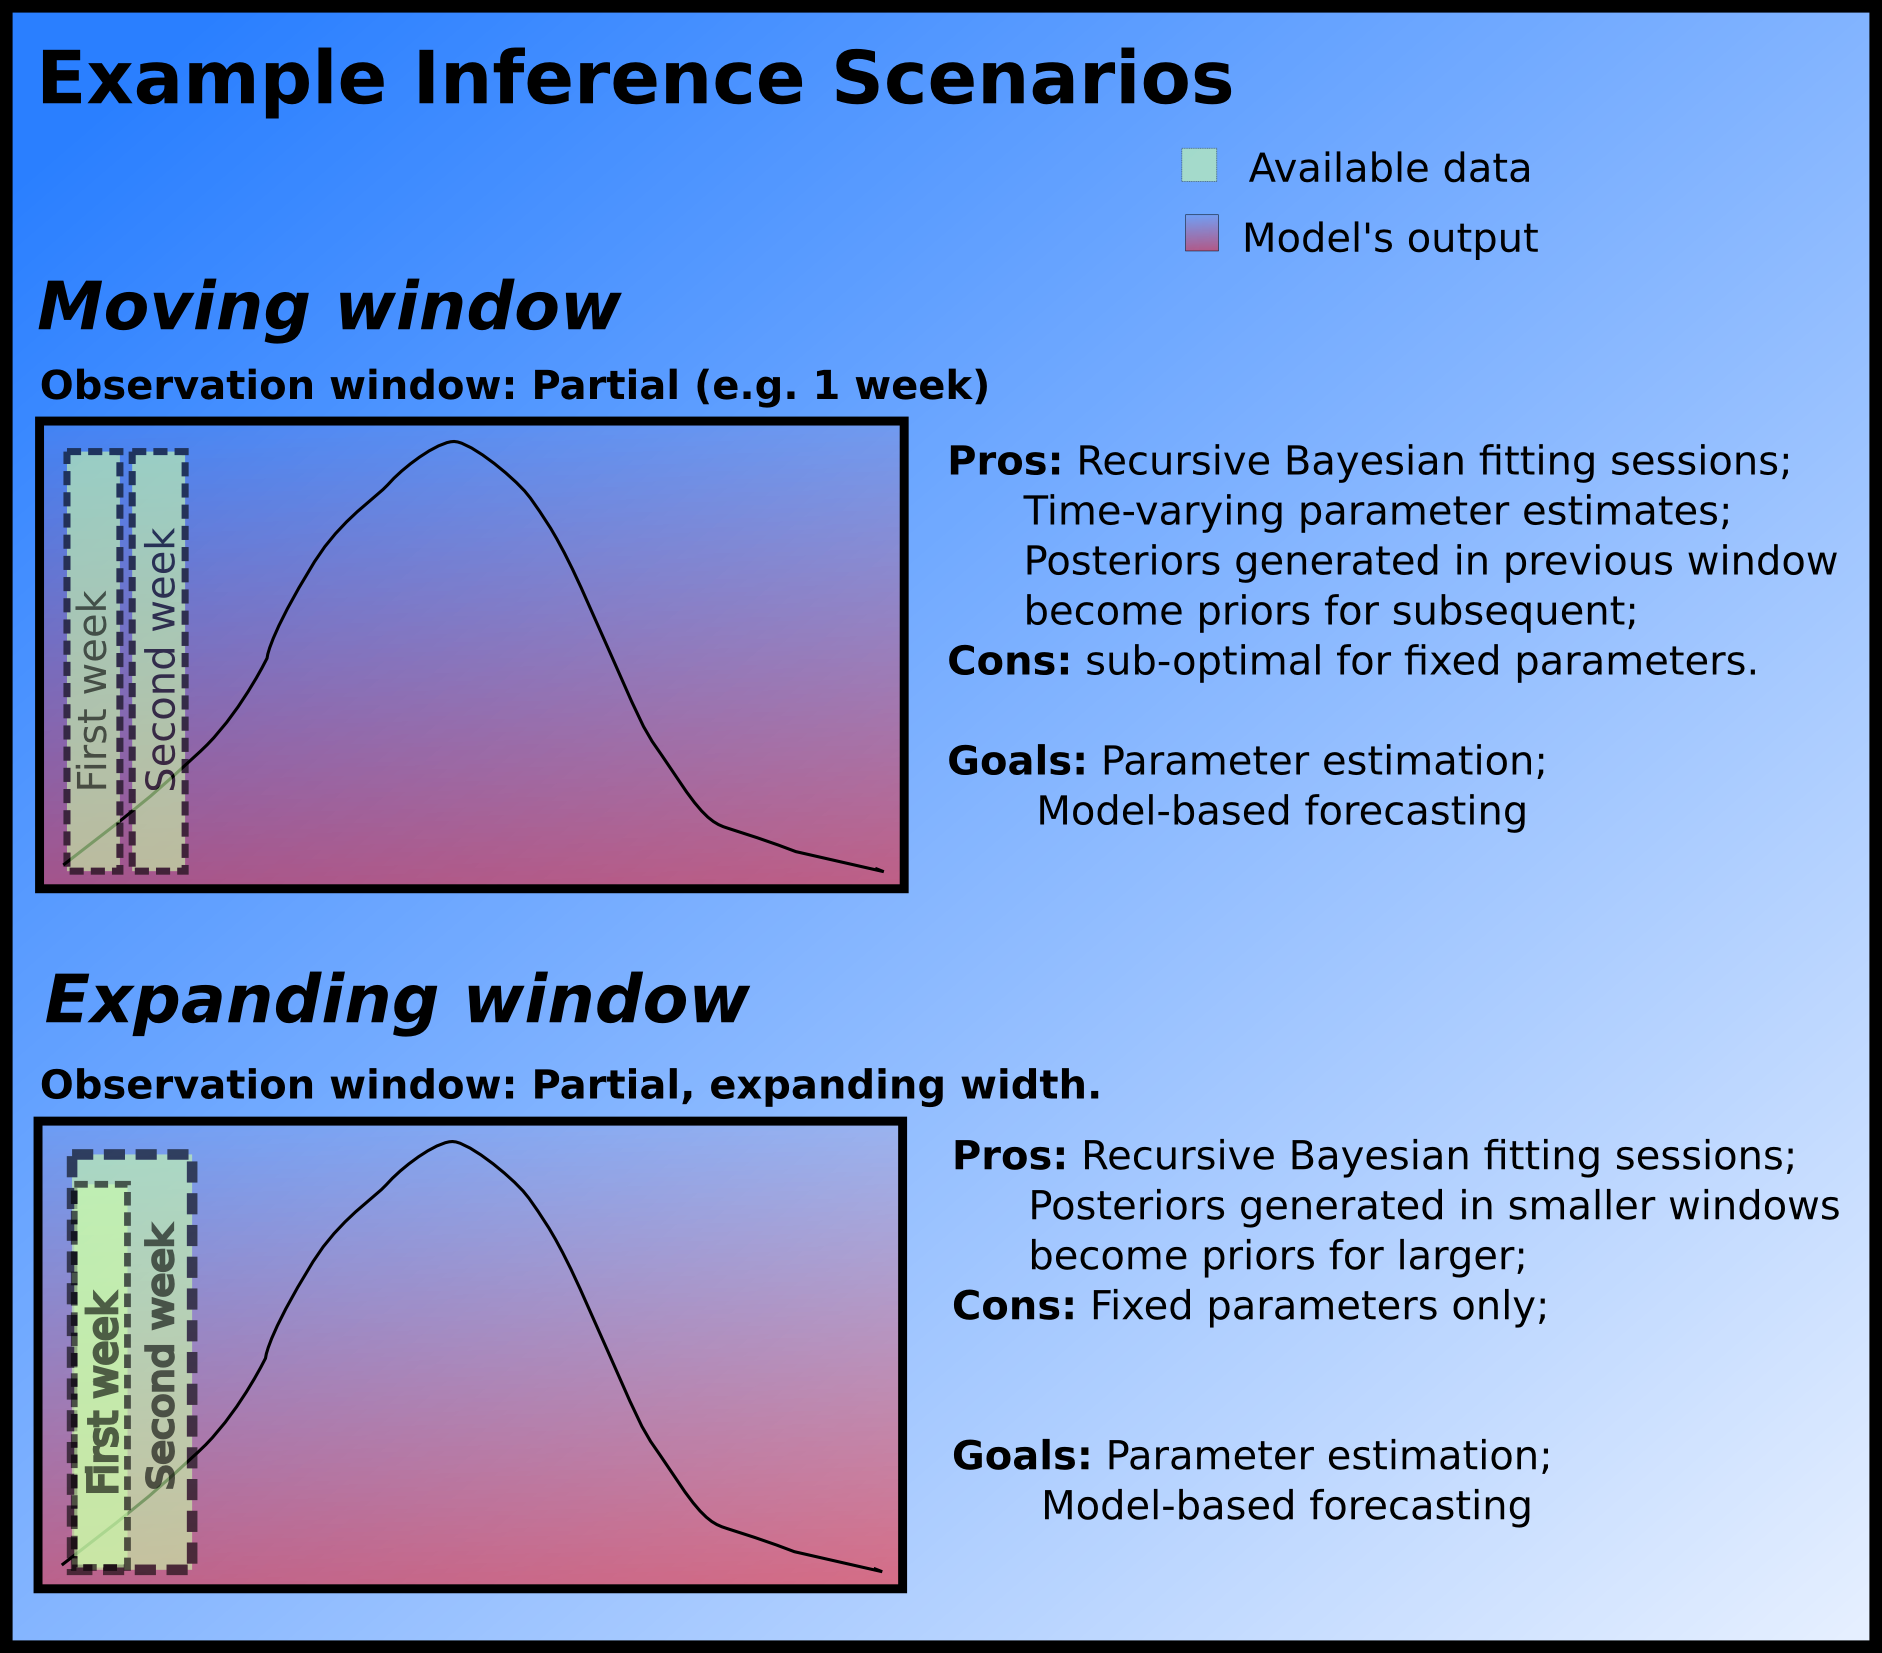
\includegraphics[width=15cm]{Inference_scenarios2.png}
\caption{Fitting scenarios: Moving windows and expanding windows.}\end{figure}


\subsection{References}
\label{paramest:references}

\section{Stochastic Differential Equations}
\label{sde:stochastic-differential-equations}\label{sde:sde}\label{sde::doc}
The SDE package in BIP, was born out of the need to simulate stochastic model to test the Parameters estimation routines in the Bayes Package. However, it is useful in many general-purpose application since it provides a pure Python implementation of an SDE solver.

Currently it provides a single solving algorithm, the Gillespie SSA. but other algorithms are planned for future releases


\chapter{Modules}
\label{index:modules}
\begin{longtable}{ll}
\hline
\endfirsthead

\multicolumn{2}{c}%
{{\textsf{\tablename\ \thetable{} -- continued from previous page}}} \\
\hline
\endhead

\hline \multicolumn{2}{|r|}{{\textsf{Continued on next page}}} \\ \hline
\endfoot

\endlastfoot


{\hyperref[BIP:module-BIP]{\code{BIP}}}
 & 
Bayesian Inference Package containing usefull classes and functions for doing inference in various applications.
\\

{\hyperref[BIP.Bayes:module-BIP.Bayes]{\code{BIP.Bayes}}}
 & 
Basic Likelihood tools such as functions for computing likelihoods, Latin Hypercube sampling (efficient random sampling) and other tools which don't belong on other packages, or apply to multiple packages.
\\

{\hyperref[BIP.Bayes.Samplers:module-BIP.Bayes.Samplers]{\code{BIP.Bayes.Samplers}}}
 & 

\\
\hline\end{longtable}



\section{BIP}
\label{BIP:module-BIP}\label{BIP::doc}\label{BIP:bip}\index{BIP (module)}
Bayesian Inference Package containing usefull classes and functions
for doing inference in various applications.

This is not a ``Bayesian Statistics'' package, i.e., it was not conceived  
to provide data analysis methods such as the one you can find 
on a statistical package such as R (for example).

Here, you will find some the basic building blocks those 
sophisticated Bayesian regression methods are built from, such as 
likelihood functions, MCMC samplers, SMC samplers, etc..

This package exists because such basic tools are not readily accessible 
in Task-oriented statistical software. From these tools, as this package matures,
you will be able to easily build a solution for your own inferential inquiries, 
a solution which may not be available on standard statistical packages.
\paragraph{Classes}

\begin{longtable}{ll}
\hline
\endfirsthead

\multicolumn{2}{c}%
{{\textsf{\tablename\ \thetable{} -- continued from previous page}}} \\
\hline
\endhead

\hline \multicolumn{2}{|r|}{{\textsf{Continued on next page}}} \\ \hline
\endfoot

\endlastfoot


\code{RotatingFileHandler}(filename{[}, mode, ...{]})
 & 
Handler for logging to a set of files, which switches from one file to the next when the current file reaches a certain size.
\\
\hline\end{longtable}



\section{BIP.Bayes}
\label{BIP.Bayes:module-BIP.Bayes}\label{BIP.Bayes::doc}\label{BIP.Bayes:bip-bayes}\index{BIP.Bayes (module)}
Basic Likelihood tools such as functions for computing likelihoods, Latin Hypercube sampling (efficient random sampling) and other tools which don't belong on other packages, or apply to multiple packages.


\subsection{Melding Module}
\label{BIP.Bayes:module-BIP.Bayes.Melding}\label{BIP.Bayes:melding-module}\index{BIP.Bayes.Melding (module)}\index{FitModel (class in BIP.Bayes.Melding)}

\begin{fulllineitems}
\phantomsection\label{BIP.Bayes:BIP.Bayes.Melding.FitModel}\pysiglinewithargsret{\strong{class }\code{BIP.Bayes.Melding.}\bfcode{FitModel}}{\emph{K}, \emph{model}, \emph{inits}, \emph{tf}, \emph{thetanames}, \emph{phinames}, \emph{wl=None}, \emph{nw=1}, \emph{verbose=False}, \emph{burnin=1000}, \emph{constraints=}\optional{}}{}
Fit a model to data generating
Bayesian posterior distributions of input and
outputs of the model.
\index{AIC\_from\_RSS() (BIP.Bayes.Melding.FitModel method)}

\begin{fulllineitems}
\phantomsection\label{BIP.Bayes:BIP.Bayes.Melding.FitModel.AIC_from_RSS}\pysiglinewithargsret{\bfcode{AIC\_from\_RSS}}{}{}
Calculates the Akaike information criterion from the residual sum of squares 
of the best fitting run.

\end{fulllineitems}

\index{do\_inference() (BIP.Bayes.Melding.FitModel method)}

\begin{fulllineitems}
\phantomsection\label{BIP.Bayes:BIP.Bayes.Melding.FitModel.do_inference}\pysiglinewithargsret{\bfcode{do\_inference}}{\emph{prior}, \emph{data}, \emph{predlen}, \emph{method}, \emph{likvar}}{}~\begin{quote}\begin{description}
\item[{Parameters}] \leavevmode\begin{itemize}
\item {} 
\textbf{prior} -- 

\item {} 
\textbf{data} -- 

\item {} 
\textbf{predlen} -- 

\item {} 
\textbf{method} -- 

\item {} 
\textbf{likvar} -- 

\end{itemize}

\end{description}\end{quote}

\end{fulllineitems}

\index{optimize() (BIP.Bayes.Melding.FitModel method)}

\begin{fulllineitems}
\phantomsection\label{BIP.Bayes:BIP.Bayes.Melding.FitModel.optimize}\pysiglinewithargsret{\bfcode{optimize}}{\emph{data}, \emph{p0}, \emph{optimizer='scipy'}, \emph{tol=0.0001}, \emph{verbose=0}, \emph{plot=0}}{}
Finds best parameters using an optimization approach
\begin{quote}\begin{description}
\item[{Parameters}] \leavevmode\begin{itemize}
\item {} 
\emph{data}: Dictionary of observed series

\item {} 
\emph{p0}: Sequence (list or tuple) of initial values for the parameters

\item {} 
\emph{optimizer}: Optimization library to use: `scipy': fmin (Nelder-Mead) or `oo':OpenOpt.NLP

\item {} 
\emph{tol}: Tolerance of the error

\item {} 
\emph{verbose}: If true show stats of the optimization run at the end

\item {} 
\emph{plot}: If true plots a run based on the optimized parameters.

\end{itemize}

\end{description}\end{quote}

\end{fulllineitems}

\index{plot\_results() (BIP.Bayes.Melding.FitModel method)}

\begin{fulllineitems}
\phantomsection\label{BIP.Bayes:BIP.Bayes.Melding.FitModel.plot_results}\pysiglinewithargsret{\bfcode{plot\_results}}{\emph{names=}\optional{}, \emph{dbname='results'}, \emph{savefigs=0}}{}
Plot the final results of the inference

\end{fulllineitems}

\index{prior\_sample() (BIP.Bayes.Melding.FitModel method)}

\begin{fulllineitems}
\phantomsection\label{BIP.Bayes:BIP.Bayes.Melding.FitModel.prior_sample}\pysiglinewithargsret{\bfcode{prior\_sample}}{}{}
Generates a set of samples from the starting theta prior distributions
for reporting purposes.
\begin{quote}\begin{description}
\item[{Returns}] \leavevmode
Dictionary with (name,sample) pairs

\end{description}\end{quote}

\end{fulllineitems}

\index{run() (BIP.Bayes.Melding.FitModel method)}

\begin{fulllineitems}
\phantomsection\label{BIP.Bayes:BIP.Bayes.Melding.FitModel.run}\pysiglinewithargsret{\bfcode{run}}{\emph{data}, \emph{method}, \emph{likvar}, \emph{pool=False}, \emph{adjinits=True}, \emph{ew=0}, \emph{dbname='results'}, \emph{monitor=False}, \emph{initheta=}\optional{}}{}
Fit the model against data
\begin{quote}\begin{description}
\item[{Parameters}] \leavevmode\begin{itemize}
\item {} 
\emph{data}: dictionary with variable names and observed series, as Key and value respectively.

\item {} 
\emph{method}: Inference method: ``ABC'', ``SIR'', ``MCMC'' or ``DREAM''

\item {} 
\emph{likvar}: Variance of the likelihood function in the SIR and MCMC method

\item {} 
\emph{pool}: Pool priors on model's outputs.

\item {} 
\emph{adjinits}: whether to adjust inits to data

\item {} 
\emph{ew}: Whether to use expanding windows instead of moving ones.

\item {} 
\emph{dbname}: name of the sqlite3 database

\item {} 
\emph{monitor}: Whether to monitor certains variables during the inference. If not False, should be a list of valid phi variable names.

\item {} 
\emph{initheta}: starting position in parameter space for the sampling to start. (only used by MCMC and DREAM)

\end{itemize}

\end{description}\end{quote}

\end{fulllineitems}

\index{set\_priors() (BIP.Bayes.Melding.FitModel method)}

\begin{fulllineitems}
\phantomsection\label{BIP.Bayes:BIP.Bayes.Melding.FitModel.set_priors}\pysiglinewithargsret{\bfcode{set\_priors}}{\emph{tdists}, \emph{tpars}, \emph{tlims}, \emph{pdists}, \emph{ppars}, \emph{plims}}{}
Set the prior distributions for Phi and Theta
\begin{quote}\begin{description}
\item[{Parameters}] \leavevmode\begin{itemize}
\item {} 
\emph{pdists}: distributions for the output variables. For example: {[}scipy.stats.uniform,scipy.stats.norm{]}

\item {} 
\emph{ppars}: paramenters for the distributions in pdists. For example: {[}(0,1),(0,1){]}

\item {} 
\emph{plims}: Limits of the range of each phi. List of (min,max) tuples.

\item {} 
\emph{tdists}: same as pdists, but for input parameters (Theta).

\item {} 
\emph{tpars}: same as ppars, but for tdists.

\item {} 
\emph{tlims}: Limits of the range of each theta. List of (min,max) tuples.

\end{itemize}

\end{description}\end{quote}

\end{fulllineitems}


\end{fulllineitems}

\index{Meld (class in BIP.Bayes.Melding)}

\begin{fulllineitems}
\phantomsection\label{BIP.Bayes:BIP.Bayes.Melding.Meld}\pysiglinewithargsret{\strong{class }\code{BIP.Bayes.Melding.}\bfcode{Meld}}{\emph{K}, \emph{L}, \emph{model}, \emph{ntheta}, \emph{nphi}, \emph{alpha=0.5}, \emph{verbose=0}, \emph{viz=False}}{}
Bayesian Melding class
\index{abcRun() (BIP.Bayes.Melding.Meld method)}

\begin{fulllineitems}
\phantomsection\label{BIP.Bayes:BIP.Bayes.Melding.Meld.abcRun}\pysiglinewithargsret{\bfcode{abcRun}}{\emph{fitfun=None}, \emph{data=\{\}}, \emph{t=1}, \emph{pool=False}, \emph{savetemp=False}}{}
Runs the model for inference through Approximate Bayes Computation
techniques. This method should be used as an alternative to the sir.
\begin{quote}\begin{description}
\item[{Parameters}] \leavevmode\begin{itemize}
\item {} 
\emph{fitfun}: Callable which will return the goodness of fit of the model to data as a number between 0-1, with 1 meaning perfect fit

\item {} 
\emph{t}: number of time steps to retain at the end of the of the model run for fitting purposes.

\item {} 
\emph{data}: dict containing observed time series (lists of length t) of the state variables. This dict must have as many items the number of state variables, with labels matching variables names. Unorbserved variables must have an empty list as value.

\item {} 
\emph{pool}: if True, Pools the user provided priors on the model's outputs, with the model induced priors.

\item {} 
\emph{savetemp}: Should temp results be saved. Useful for long runs. Alows for resuming the simulation from last sa

\end{itemize}

\end{description}\end{quote}

\end{fulllineitems}

\index{add\_salt() (BIP.Bayes.Melding.Meld method)}

\begin{fulllineitems}
\phantomsection\label{BIP.Bayes:BIP.Bayes.Melding.Meld.add_salt}\pysiglinewithargsret{\bfcode{add\_salt}}{\emph{dataset}, \emph{band}}{}
Adds a few extra uniformly distributed data 
points beyond the dataset range.
This is done by adding from a uniform dist.
\begin{quote}\begin{description}
\item[{Parameters}] \leavevmode\begin{itemize}
\item {} 
\emph{dataset}: vector of data

\item {} 
\emph{band}: Fraction of range to extend {[}0,1{[}

\end{itemize}

\item[{Returns}] \leavevmode
Salted dataset.

\end{description}\end{quote}

\end{fulllineitems}

\index{current\_plot() (BIP.Bayes.Melding.Meld method)}

\begin{fulllineitems}
\phantomsection\label{BIP.Bayes:BIP.Bayes.Melding.Meld.current_plot}\pysiglinewithargsret{\bfcode{current\_plot}}{\emph{series}, \emph{data}, \emph{idx}, \emph{vars=}\optional{}, \emph{step=0}}{}
Plots the last simulated series
\begin{quote}
\begin{quote}\begin{description}
\item[{Parameters}] \leavevmode\begin{itemize}
\item {} 
\emph{series}: Record array with the simulated series.

\item {} 
\emph{idx}: Integer index of the curve to plot .

\item {} 
\emph{data}: Dictionary with the full dataset.

\item {} 
\emph{vars}: List with variable names to be plotted.

\item {} 
\emph{step}: Step of the chain

\end{itemize}

\end{description}\end{quote}
\end{quote}

\end{fulllineitems}

\index{filtM() (BIP.Bayes.Melding.Meld method)}

\begin{fulllineitems}
\phantomsection\label{BIP.Bayes:BIP.Bayes.Melding.Meld.filtM}\pysiglinewithargsret{\bfcode{filtM}}{\emph{cond}, \emph{x}, \emph{limits}}{}
Multiple condition filtering.
Remove values in x{[}i{]}, if corresponding values in
cond{[}i{]} are less than limits{[}i{]}{[}0{]} or greater than
limits{[}i{]}{[}1{]}.
\begin{quote}\begin{description}
\item[{Parameters}] \leavevmode\begin{itemize}
\item {} 
\emph{cond}: is an array of conditions.

\item {} 
\emph{limits}: is a list of tuples (ll,ul) with length equal to number of lines in \emph{cond} and \emph{x}.

\item {} 
\emph{x}: array to be filtered.

\end{itemize}

\end{description}\end{quote}

\end{fulllineitems}

\index{getPosteriors() (BIP.Bayes.Melding.Meld method)}

\begin{fulllineitems}
\phantomsection\label{BIP.Bayes:BIP.Bayes.Melding.Meld.getPosteriors}\pysiglinewithargsret{\bfcode{getPosteriors}}{\emph{t}}{}
Updates the posteriors of the model's output for the last t time steps.
Returns two record arrays:
- The posteriors of the Theta
- the posterior of Phi last t values of time-series. self.L by \emph{t} arrays.
\begin{quote}\begin{description}
\item[{Parameters}] \leavevmode\begin{itemize}
\item {} 
\emph{t}: length of the posterior time-series to return.

\end{itemize}

\end{description}\end{quote}

\end{fulllineitems}

\index{imp\_sample() (BIP.Bayes.Melding.Meld method)}

\begin{fulllineitems}
\phantomsection\label{BIP.Bayes:BIP.Bayes.Melding.Meld.imp_sample}\pysiglinewithargsret{\bfcode{imp\_sample}}{\emph{n}, \emph{data}, \emph{w}}{}
Importance sampling
\begin{quote}\begin{description}
\item[{Returns}] \leavevmode
returns a sample of size n

\end{description}\end{quote}

\end{fulllineitems}

\index{logPooling() (BIP.Bayes.Melding.Meld method)}

\begin{fulllineitems}
\phantomsection\label{BIP.Bayes:BIP.Bayes.Melding.Meld.logPooling}\pysiglinewithargsret{\bfcode{logPooling}}{\emph{phi}}{}
Returns the probability associated with each phi{[}i{]}
on the pooled pdf of phi and q2phi.
\begin{quote}\begin{description}
\item[{Parameters}] \leavevmode\begin{itemize}
\item {} 
\emph{phi}: prior of Phi induced by the model and q1theta.

\end{itemize}

\end{description}\end{quote}

\end{fulllineitems}

\index{mcmc\_run() (BIP.Bayes.Melding.Meld method)}

\begin{fulllineitems}
\phantomsection\label{BIP.Bayes:BIP.Bayes.Melding.Meld.mcmc_run}\pysiglinewithargsret{\bfcode{mcmc\_run}}{\emph{data}, \emph{t=1}, \emph{likvariance=10}, \emph{burnin=1000}, \emph{nopool=False}, \emph{method='MH'}, \emph{constraints=}\optional{}}{}
MCMC based fitting
\begin{quote}\begin{description}
\item[{Parameters}] \leavevmode\begin{itemize}
\item {} 
\emph{data}: observed time series on the model's output

\item {} 
\emph{t}: length of the observed time series

\item {} 
\emph{likvariance}: variance of the Normal likelihood function

\item {} 
\emph{nopool}: True if no priors on the outputs are available. Leads to faster calculations

\item {} 
\emph{method}: Step method. defaults to Metropolis hastings

\end{itemize}

\end{description}\end{quote}

\end{fulllineitems}

\index{run() (BIP.Bayes.Melding.Meld method)}

\begin{fulllineitems}
\phantomsection\label{BIP.Bayes:BIP.Bayes.Melding.Meld.run}\pysiglinewithargsret{\bfcode{run}}{\emph{*args}}{}
Runs the model through the Melding inference.model
model is a callable which return the output of the deterministic model,
i.e. the model itself.
The model is run self.K times to obtain phi = M(theta).

\end{fulllineitems}

\index{runModel() (BIP.Bayes.Melding.Meld method)}

\begin{fulllineitems}
\phantomsection\label{BIP.Bayes:BIP.Bayes.Melding.Meld.runModel}\pysiglinewithargsret{\bfcode{runModel}}{\emph{savetemp}, \emph{t=1}, \emph{k=None}}{}
Handles running the model k times keeping a temporary savefile for
resuming calculation in case of interruption.
\begin{quote}\begin{description}
\item[{Parameters}] \leavevmode\begin{itemize}
\item {} 
\emph{savetemp}: Boolean. create a temp file?

\item {} 
\emph{t}: number of time steps

\end{itemize}

\item[{Returns}] \leavevmode\begin{itemize}
\item {} 
self.phi: a record array of shape (k,t) with the results.

\end{itemize}

\end{description}\end{quote}

\end{fulllineitems}

\index{setPhi() (BIP.Bayes.Melding.Meld method)}

\begin{fulllineitems}
\phantomsection\label{BIP.Bayes:BIP.Bayes.Melding.Meld.setPhi}\pysiglinewithargsret{\bfcode{setPhi}}{\emph{names, dists={[}\textless{}scipy.stats.\_continuous\_distns.norm\_gen object at 0x411ebd0\textgreater{}{]}, pars={[}(0, 1){]}, limits={[}(-5, 5){]}}}{}
Setup the models Outputs, or Phi, and generate the samples from prior distributions 
needed for the melding replicates.
\begin{quote}\begin{description}
\item[{Parameters}] \leavevmode\begin{itemize}
\item {} 
\emph{names}: list of string with the names of the variables.

\item {} 
\emph{dists}: is a list of RNG from scipy.stats

\item {} 
\emph{pars}: is a list of tuples of variables for each prior distribution, respectively.

\item {} 
\emph{limits}: lower and upper limits on the support of variables.

\end{itemize}

\end{description}\end{quote}

\end{fulllineitems}

\index{setPhiFromData() (BIP.Bayes.Melding.Meld method)}

\begin{fulllineitems}
\phantomsection\label{BIP.Bayes:BIP.Bayes.Melding.Meld.setPhiFromData}\pysiglinewithargsret{\bfcode{setPhiFromData}}{\emph{names}, \emph{data}, \emph{limits}}{}
Setup the model outputs and set their prior distributions from the
vectors in data.
This method is to be used when the prior distributions are available in
the form of a sample from an empirical distribution such as a bayesian
posterior.
In order to expand the samples provided, K samples are generated from a
kernel density estimate of the original sample.
\begin{quote}\begin{description}
\item[{Parameters}] \leavevmode\begin{itemize}
\item {} 
\emph{names}: list of string with the names of the variables.

\item {} 
\emph{data}: list of vectors. Samples of the proposed distribution.

\item {} 
\emph{limits}: list of tuples (ll,ul),lower and upper limits on the support of variables.

\end{itemize}

\end{description}\end{quote}

\end{fulllineitems}

\index{setTheta() (BIP.Bayes.Melding.Meld method)}

\begin{fulllineitems}
\phantomsection\label{BIP.Bayes:BIP.Bayes.Melding.Meld.setTheta}\pysiglinewithargsret{\bfcode{setTheta}}{\emph{names, dists={[}\textless{}scipy.stats.\_continuous\_distns.norm\_gen object at 0x411ebd0\textgreater{}{]}, pars={[}(0, 1){]}, lims={[}(0, 1){]}}}{}
Setup the models inputs and generate the samples from prior distributions 
needed for the dists the melding replicates.
\begin{quote}\begin{description}
\item[{Parameters}] \leavevmode\begin{itemize}
\item {} 
\emph{names}: list of string with the names of the parameters.

\item {} 
\emph{dists}: is a list of RNG from scipy.stats

\item {} 
\emph{pars}: is a list of tuples of parameters for each prior distribution, respectivelydists

\end{itemize}

\end{description}\end{quote}

\end{fulllineitems}

\index{setThetaFromData() (BIP.Bayes.Melding.Meld method)}

\begin{fulllineitems}
\phantomsection\label{BIP.Bayes:BIP.Bayes.Melding.Meld.setThetaFromData}\pysiglinewithargsret{\bfcode{setThetaFromData}}{\emph{names}, \emph{data}, \emph{limits}}{}
Setup the model inputs and set the prior distributions from the vectors
in data.
This method is to be used when the prior distributions are available in 
the form of a sample from an empirical distribution such as a bayesian
posterior.
In order to expand the samples provided, K samples are generated from a
kernel density estimate of the original sample.
\begin{quote}\begin{description}
\item[{Parameters}] \leavevmode\begin{itemize}
\item {} 
\emph{names}: list of string with the names of the parameters.

\item {} 
\emph{data}: list of vectors. Samples of a proposed distribution

\item {} 
\emph{limits}: List of (min,max) tuples for each theta to make sure samples are not generated outside these limits.

\end{itemize}

\end{description}\end{quote}

\end{fulllineitems}

\index{sir() (BIP.Bayes.Melding.Meld method)}

\begin{fulllineitems}
\phantomsection\label{BIP.Bayes:BIP.Bayes.Melding.Meld.sir}\pysiglinewithargsret{\bfcode{sir}}{\emph{data=\{\}}, \emph{t=1}, \emph{variance=0.1}, \emph{pool=False}, \emph{savetemp=False}}{}
Run the model output through the Sampling-Importance-Resampling algorithm.
Returns 1 if successful or 0 if not.
\begin{quote}\begin{description}
\item[{Parameters}] \leavevmode\begin{itemize}
\item {} 
\emph{data}: observed time series on the model's output

\item {} 
\emph{t}: length of the observed time series

\item {} 
\emph{variance}: variance of the Normal likelihood function

\item {} 
\emph{pool}: False if no priors on the outputs are available. Leads to faster calculations

\item {} 
\emph{savetemp}: Boolean. create a temp file?

\end{itemize}

\end{description}\end{quote}

\end{fulllineitems}


\end{fulllineitems}

\index{basicfit() (in module BIP.Bayes.Melding)}

\begin{fulllineitems}
\phantomsection\label{BIP.Bayes:BIP.Bayes.Melding.basicfit}\pysiglinewithargsret{\code{BIP.Bayes.Melding.}\bfcode{basicfit}}{\emph{s1}, \emph{s2}}{}
Calculates a basic fitness calculation between a model-
generated time series and a observed time series.
it uses a Mean square error.
\begin{quote}\begin{description}
\item[{Parameters}] \leavevmode\begin{itemize}
\item {} 
\emph{s1}: model-generated time series. record array.

\item {} 
\emph{s2}: observed time series. dictionary with keys matching names of s1

\end{itemize}

\item[{Return}] \leavevmode
Root mean square deviation between ´s1´ and ´s2´.

\end{description}\end{quote}

\end{fulllineitems}

\index{clearNaN() (in module BIP.Bayes.Melding)}

\begin{fulllineitems}
\phantomsection\label{BIP.Bayes:BIP.Bayes.Melding.clearNaN}\pysiglinewithargsret{\code{BIP.Bayes.Melding.}\bfcode{clearNaN}}{\emph{obs}}{}
Loops through an array with data series as columns, and 
Replaces NaNs with the mean of the other series.
\begin{quote}\begin{description}
\item[{Parameters}] \leavevmode\begin{itemize}
\item {} 
\emph{obs}: 2-dimensional numpy array

\end{itemize}

\item[{Returns}] \leavevmode
array of the same shape as obs

\end{description}\end{quote}

\end{fulllineitems}

\index{enumRun() (in module BIP.Bayes.Melding)}

\begin{fulllineitems}
\phantomsection\label{BIP.Bayes:BIP.Bayes.Melding.enumRun}\pysiglinewithargsret{\code{BIP.Bayes.Melding.}\bfcode{enumRun}}{\emph{model}, \emph{theta}, \emph{k}}{}
Returns model results plus run number.
\begin{quote}\begin{description}
\item[{Parameters}] \leavevmode\begin{itemize}
\item {} 
\emph{model}: model callable

\item {} 
\emph{theta}: model input list

\item {} 
\emph{k}: run number

\end{itemize}

\item[{Return}] \leavevmode\begin{itemize}
\item {} 
res: result list

\item {} 
\emph{k}: run number

\end{itemize}

\end{description}\end{quote}

\end{fulllineitems}

\index{model() (in module BIP.Bayes.Melding)}

\begin{fulllineitems}
\phantomsection\label{BIP.Bayes:BIP.Bayes.Melding.model}\pysiglinewithargsret{\code{BIP.Bayes.Melding.}\bfcode{model}}{\emph{theta}, \emph{n=1}}{}
Model (r,p0, n=1)
Simulates the Population dynamic Model (PDM) Pt = rP0
for n time steps.
P0 is the initial population size. 
Example model for testing purposes.

\end{fulllineitems}

\index{model\_as\_ra() (in module BIP.Bayes.Melding)}

\begin{fulllineitems}
\phantomsection\label{BIP.Bayes:BIP.Bayes.Melding.model_as_ra}\pysiglinewithargsret{\code{BIP.Bayes.Melding.}\bfcode{model\_as\_ra}}{\emph{theta}, \emph{model}, \emph{phinames}}{}
Does a single run of self.model and returns the results as a record array

\end{fulllineitems}

\index{plotRaHist() (in module BIP.Bayes.Melding)}

\begin{fulllineitems}
\phantomsection\label{BIP.Bayes:BIP.Bayes.Melding.plotRaHist}\pysiglinewithargsret{\code{BIP.Bayes.Melding.}\bfcode{plotRaHist}}{\emph{arr}}{}
Plots a record array
as a panel of histograms

\end{fulllineitems}

\index{randint() (in module BIP.Bayes.Melding)}

\begin{fulllineitems}
\phantomsection\label{BIP.Bayes:BIP.Bayes.Melding.randint}\pysiglinewithargsret{\code{BIP.Bayes.Melding.}\bfcode{randint}}{\emph{low}, \emph{high=None}, \emph{size=None}}{}
Return random integers from \emph{low} (inclusive) to \emph{high} (exclusive).

Return random integers from the ``discrete uniform'' distribution in the
``half-open'' interval {[}\emph{low}, \emph{high}). If \emph{high} is None (the default),
then results are from {[}0, \emph{low}).
\begin{description}
\item[{low}] \leavevmode{[}int{]}
Lowest (signed) integer to be drawn from the distribution (unless
\code{high=None}, in which case this parameter is the \emph{highest} such
integer).

\item[{high}] \leavevmode{[}int, optional{]}
If provided, one above the largest (signed) integer to be drawn
from the distribution (see above for behavior if \code{high=None}).

\item[{size}] \leavevmode{[}int or tuple of ints, optional{]}
Output shape. Default is None, in which case a single int is
returned.

\end{description}
\begin{description}
\item[{out}] \leavevmode{[}int or ndarray of ints{]}
\emph{size}-shaped array of random integers from the appropriate
distribution, or a single such random int if \emph{size} not provided.

\end{description}
\begin{description}
\item[{random.random\_integers}] \leavevmode{[}similar to \emph{randint}, only for the closed{]}
interval {[}\emph{low}, \emph{high}{]}, and 1 is the lowest value if \emph{high} is
omitted. In particular, this other one is the one to use to generate
uniformly distributed discrete non-integers.

\end{description}

\begin{Verbatim}[commandchars=\\\{\}]
\PYG{g+gp}{\PYGZgt{}\PYGZgt{}\PYGZgt{} }\PYG{n}{np}\PYG{o}{.}\PYG{n}{random}\PYG{o}{.}\PYG{n}{randint}\PYG{p}{(}\PYG{l+m+mi}{2}\PYG{p}{,} \PYG{n}{size}\PYG{o}{=}\PYG{l+m+mi}{10}\PYG{p}{)}
\PYG{g+go}{array([1, 0, 0, 0, 1, 1, 0, 0, 1, 0])}
\PYG{g+gp}{\PYGZgt{}\PYGZgt{}\PYGZgt{} }\PYG{n}{np}\PYG{o}{.}\PYG{n}{random}\PYG{o}{.}\PYG{n}{randint}\PYG{p}{(}\PYG{l+m+mi}{1}\PYG{p}{,} \PYG{n}{size}\PYG{o}{=}\PYG{l+m+mi}{10}\PYG{p}{)}
\PYG{g+go}{array([0, 0, 0, 0, 0, 0, 0, 0, 0, 0])}
\end{Verbatim}

Generate a 2 x 4 array of ints between 0 and 4, inclusive:

\begin{Verbatim}[commandchars=\\\{\}]
\PYG{g+gp}{\PYGZgt{}\PYGZgt{}\PYGZgt{} }\PYG{n}{np}\PYG{o}{.}\PYG{n}{random}\PYG{o}{.}\PYG{n}{randint}\PYG{p}{(}\PYG{l+m+mi}{5}\PYG{p}{,} \PYG{n}{size}\PYG{o}{=}\PYG{p}{(}\PYG{l+m+mi}{2}\PYG{p}{,} \PYG{l+m+mi}{4}\PYG{p}{)}\PYG{p}{)}
\PYG{g+go}{array([[4, 0, 2, 1],}
\PYG{g+go}{       [3, 2, 2, 0]])}
\end{Verbatim}

\end{fulllineitems}

\index{random() (in module BIP.Bayes.Melding)}

\begin{fulllineitems}
\phantomsection\label{BIP.Bayes:BIP.Bayes.Melding.random}\pysiglinewithargsret{\code{BIP.Bayes.Melding.}\bfcode{random}}{}{}
random\_sample(size=None)

Return random floats in the half-open interval {[}0.0, 1.0).

Results are from the ``continuous uniform'' distribution over the
stated interval.  To sample \(Unif[a, b), b > a\) multiply
the output of \emph{random\_sample} by \emph{(b-a)} and add \emph{a}:

\begin{Verbatim}[commandchars=\\\{\}]
\PYG{p}{(}\PYG{n}{b} \PYG{o}{\PYGZhy{}} \PYG{n}{a}\PYG{p}{)} \PYG{o}{*} \PYG{n}{random\PYGZus{}sample}\PYG{p}{(}\PYG{p}{)} \PYG{o}{+} \PYG{n}{a}
\end{Verbatim}
\begin{description}
\item[{size}] \leavevmode{[}int or tuple of ints, optional{]}
Defines the shape of the returned array of random floats. If None
(the default), returns a single float.

\end{description}
\begin{description}
\item[{out}] \leavevmode{[}float or ndarray of floats{]}
Array of random floats of shape \emph{size} (unless \code{size=None}, in which
case a single float is returned).

\end{description}

\begin{Verbatim}[commandchars=\\\{\}]
\PYG{g+gp}{\PYGZgt{}\PYGZgt{}\PYGZgt{} }\PYG{n}{np}\PYG{o}{.}\PYG{n}{random}\PYG{o}{.}\PYG{n}{random\PYGZus{}sample}\PYG{p}{(}\PYG{p}{)}
\PYG{g+go}{0.47108547995356098}
\PYG{g+gp}{\PYGZgt{}\PYGZgt{}\PYGZgt{} }\PYG{n+nb}{type}\PYG{p}{(}\PYG{n}{np}\PYG{o}{.}\PYG{n}{random}\PYG{o}{.}\PYG{n}{random\PYGZus{}sample}\PYG{p}{(}\PYG{p}{)}\PYG{p}{)}
\PYG{g+go}{\PYGZlt{}type \PYGZsq{}float\PYGZsq{}\PYGZgt{}}
\PYG{g+gp}{\PYGZgt{}\PYGZgt{}\PYGZgt{} }\PYG{n}{np}\PYG{o}{.}\PYG{n}{random}\PYG{o}{.}\PYG{n}{random\PYGZus{}sample}\PYG{p}{(}\PYG{p}{(}\PYG{l+m+mi}{5}\PYG{p}{,}\PYG{p}{)}\PYG{p}{)}
\PYG{g+go}{array([ 0.30220482,  0.86820401,  0.1654503 ,  0.11659149,  0.54323428])}
\end{Verbatim}

Three-by-two array of random numbers from {[}-5, 0):

\begin{Verbatim}[commandchars=\\\{\}]
\PYG{g+gp}{\PYGZgt{}\PYGZgt{}\PYGZgt{} }\PYG{l+m+mi}{5} \PYG{o}{*} \PYG{n}{np}\PYG{o}{.}\PYG{n}{random}\PYG{o}{.}\PYG{n}{random\PYGZus{}sample}\PYG{p}{(}\PYG{p}{(}\PYG{l+m+mi}{3}\PYG{p}{,} \PYG{l+m+mi}{2}\PYG{p}{)}\PYG{p}{)} \PYG{o}{\PYGZhy{}} \PYG{l+m+mi}{5}
\PYG{g+go}{array([[\PYGZhy{}3.99149989, \PYGZhy{}0.52338984],}
\PYG{g+go}{       [\PYGZhy{}2.99091858, \PYGZhy{}0.79479508],}
\PYG{g+go}{       [\PYGZhy{}1.23204345, \PYGZhy{}1.75224494]])}
\end{Verbatim}

\end{fulllineitems}

\index{seed() (in module BIP.Bayes.Melding)}

\begin{fulllineitems}
\phantomsection\label{BIP.Bayes:BIP.Bayes.Melding.seed}\pysiglinewithargsret{\code{BIP.Bayes.Melding.}\bfcode{seed}}{\emph{seed=None}}{}
Seed the generator.

This method is called when \emph{RandomState} is initialized. It can be
called again to re-seed the generator. For details, see \emph{RandomState}.
\begin{description}
\item[{seed}] \leavevmode{[}int or array\_like, optional{]}
Seed for \emph{RandomState}.

\end{description}

RandomState

\end{fulllineitems}



\subsection{Log-Likelihood Functions}
\label{BIP.Bayes:log-likelihood-functions}\phantomsection\label{BIP.Bayes:module-BIP.Bayes.like}\index{BIP.Bayes.like (module)}\index{Bernoulli() (in module BIP.Bayes.like)}

\begin{fulllineitems}
\phantomsection\label{BIP.Bayes:BIP.Bayes.like.Bernoulli}\pysiglinewithargsret{\code{BIP.Bayes.like.}\bfcode{Bernoulli}}{\emph{x}, \emph{p}}{}
Log-Like Bernoulli
\textgreater{}\textgreater{}\textgreater{} Bernoulli({[}0,1,1,1,0,0,1,1{]},0.5)
-5.54517744448

\end{fulllineitems}

\index{Beta() (in module BIP.Bayes.like)}

\begin{fulllineitems}
\phantomsection\label{BIP.Bayes:BIP.Bayes.like.Beta}\pysiglinewithargsret{\code{BIP.Bayes.like.}\bfcode{Beta}}{\emph{x}, \emph{a}, \emph{b}}{}
Log-Like Beta
\textgreater{}\textgreater{}\textgreater{} Beta({[}.2,.3,.7,.6,.4{]},2,5)
-0.434845728904

\end{fulllineitems}

\index{Binomial() (in module BIP.Bayes.like)}

\begin{fulllineitems}
\phantomsection\label{BIP.Bayes:BIP.Bayes.like.Binomial}\pysiglinewithargsret{\code{BIP.Bayes.like.}\bfcode{Binomial}}{\emph{x}, \emph{n}, \emph{p}}{}
Binomial Log-Likelihood 
\textgreater{}\textgreater{}\textgreater{} Binomial({[}2,3{]},6,0.3)
-2.81280615454

\end{fulllineitems}

\index{Categor() (in module BIP.Bayes.like)}

\begin{fulllineitems}
\phantomsection\label{BIP.Bayes:BIP.Bayes.like.Categor}\pysiglinewithargsret{\code{BIP.Bayes.like.}\bfcode{Categor}}{\emph{x}, \emph{hist}}{}
Categorical Log-likelihood
generalization of a Bernoulli process for variables with any constant
number of discrete values.
\begin{quote}\begin{description}
\item[{Parameters}] \leavevmode\begin{itemize}
\item {} 
\emph{x}: data vector (list)

\item {} 
\emph{hist}: tuple (prob,classes) classes contain the superior limit of the histogram classes

\end{itemize}

\end{description}\end{quote}

\begin{Verbatim}[commandchars=\\\{\}]
\PYG{g+gp}{\PYGZgt{}\PYGZgt{}\PYGZgt{} }\PYG{n}{Categor}\PYG{p}{(}\PYG{p}{[}\PYG{l+m+mi}{1}\PYG{p}{]}\PYG{p}{,}\PYG{p}{(}\PYG{p}{[}\PYG{o}{.}\PYG{l+m+mi}{3}\PYG{p}{,}\PYG{o}{.}\PYG{l+m+mi}{7}\PYG{p}{]}\PYG{p}{,}\PYG{p}{[}\PYG{l+m+mi}{0}\PYG{p}{,}\PYG{l+m+mi}{1}\PYG{p}{]}\PYG{p}{)}\PYG{p}{)}
\PYG{g+go}{\PYGZhy{}0.356674943939}
\end{Verbatim}

\end{fulllineitems}

\index{Gamma() (in module BIP.Bayes.like)}

\begin{fulllineitems}
\phantomsection\label{BIP.Bayes:BIP.Bayes.like.Gamma}\pysiglinewithargsret{\code{BIP.Bayes.like.}\bfcode{Gamma}}{\emph{x}, \emph{alpha}, \emph{beta}}{}
Log-Like Gamma
\textgreater{}\textgreater{}\textgreater{} Gamma({[}2,3,7,6,4{]},2,2)
-11.015748357

\end{fulllineitems}

\index{Lognormal() (in module BIP.Bayes.like)}

\begin{fulllineitems}
\phantomsection\label{BIP.Bayes:BIP.Bayes.like.Lognormal}\pysiglinewithargsret{\code{BIP.Bayes.like.}\bfcode{Lognormal}}{\emph{x}, \emph{mu}, \emph{tau}}{}
Lognormal Log-likelihood
\begin{quote}\begin{description}
\item[{Parameters}] \leavevmode\begin{itemize}
\item {} 
\emph{mu}: mean

\item {} 
\emph{tau}: precision (1/sd)

\end{itemize}

\end{description}\end{quote}

\begin{Verbatim}[commandchars=\\\{\}]
\PYG{g+gp}{\PYGZgt{}\PYGZgt{}\PYGZgt{} }\PYG{n}{Lognormal}\PYG{p}{(}\PYG{p}{[}\PYG{l+m+mf}{0.5}\PYG{p}{,}\PYG{l+m+mi}{1}\PYG{p}{,}\PYG{l+m+mf}{1.2}\PYG{p}{]}\PYG{p}{,}\PYG{l+m+mi}{0}\PYG{p}{,}\PYG{l+m+mf}{0.5}\PYG{p}{)}
\PYG{g+go}{\PYGZhy{}3.15728720569}
\end{Verbatim}

\end{fulllineitems}

\index{Negbin() (in module BIP.Bayes.like)}

\begin{fulllineitems}
\phantomsection\label{BIP.Bayes:BIP.Bayes.like.Negbin}\pysiglinewithargsret{\code{BIP.Bayes.like.}\bfcode{Negbin}}{\emph{x}, \emph{r}, \emph{p}}{}
Negative Binomial Log-Likelihood 
\textgreater{}\textgreater{}\textgreater{} Negbin({[}2,3{]},6,0.3)
-9.16117424315

\end{fulllineitems}

\index{Normal() (in module BIP.Bayes.like)}

\begin{fulllineitems}
\phantomsection\label{BIP.Bayes:BIP.Bayes.like.Normal}\pysiglinewithargsret{\code{BIP.Bayes.like.}\bfcode{Normal}}{\emph{x}, \emph{mu}, \emph{tau}}{}
Normal Log-like
\begin{quote}\begin{description}
\item[{Parameters}] \leavevmode\begin{itemize}
\item {} 
\emph{mu}: mean

\item {} 
\emph{tau}: precision (1/variance)

\end{itemize}

\end{description}\end{quote}

\begin{Verbatim}[commandchars=\\\{\}]
\PYG{g+gp}{\PYGZgt{}\PYGZgt{}\PYGZgt{} }\PYG{n}{Normal}\PYG{p}{(}\PYG{p}{[}\PYG{l+m+mi}{0}\PYG{p}{]}\PYG{p}{,}\PYG{l+m+mi}{0}\PYG{p}{,}\PYG{l+m+mi}{1}\PYG{p}{)}
\PYG{g+go}{\PYGZhy{}0.918938533205}
\end{Verbatim}

\end{fulllineitems}

\index{Poisson() (in module BIP.Bayes.like)}

\begin{fulllineitems}
\phantomsection\label{BIP.Bayes:BIP.Bayes.like.Poisson}\pysiglinewithargsret{\code{BIP.Bayes.like.}\bfcode{Poisson}}{\emph{x}, \emph{mu}}{}
Poisson Log-Likelihood function 
\textgreater{}\textgreater{}\textgreater{} Poisson({[}2{]},2)
-1.30685281944

\end{fulllineitems}

\index{Simple() (in module BIP.Bayes.like)}

\begin{fulllineitems}
\phantomsection\label{BIP.Bayes:BIP.Bayes.like.Simple}\pysiglinewithargsret{\code{BIP.Bayes.like.}\bfcode{Simple}}{\emph{x}, \emph{w}, \emph{a}, \emph{start=0}}{}
find out what it is.

\end{fulllineitems}

\index{Uniform() (in module BIP.Bayes.like)}

\begin{fulllineitems}
\phantomsection\label{BIP.Bayes:BIP.Bayes.like.Uniform}\pysiglinewithargsret{\code{BIP.Bayes.like.}\bfcode{Uniform}}{\emph{x}, \emph{min}, \emph{max}}{}
Uniform Log-likelihood
\begin{quote}\begin{description}
\item[{Parameters}] \leavevmode\begin{itemize}
\item {} 
\emph{x}: data vector(list)

\item {} 
\emph{min}: lower limit of the distribution

\item {} 
\emph{max}: upper limit of the distribution

\end{itemize}

\end{description}\end{quote}

\begin{Verbatim}[commandchars=\\\{\}]
\PYG{g+gp}{\PYGZgt{}\PYGZgt{}\PYGZgt{} }\PYG{n}{Uniform}\PYG{p}{(}\PYG{p}{[}\PYG{l+m+mf}{1.1}\PYG{p}{,}\PYG{l+m+mf}{2.3}\PYG{p}{,}\PYG{l+m+mf}{3.4}\PYG{p}{,}\PYG{l+m+mi}{4}\PYG{p}{]}\PYG{p}{,}\PYG{l+m+mi}{0}\PYG{p}{,}\PYG{l+m+mi}{5}\PYG{p}{)}
\PYG{g+go}{\PYGZhy{}6.4377516497364011}
\end{Verbatim}

\end{fulllineitems}

\index{Weibull() (in module BIP.Bayes.like)}

\begin{fulllineitems}
\phantomsection\label{BIP.Bayes:BIP.Bayes.like.Weibull}\pysiglinewithargsret{\code{BIP.Bayes.like.}\bfcode{Weibull}}{\emph{x}, \emph{alpha}, \emph{beta}}{}
Log-Like Weibull
\textgreater{}\textgreater{}\textgreater{} Weibull({[}2,1,0.3,.5,1.7{]},1.5,3)
-7.811955373

\end{fulllineitems}

\index{find\_best\_tau() (in module BIP.Bayes.like)}

\begin{fulllineitems}
\phantomsection\label{BIP.Bayes:BIP.Bayes.like.find_best_tau}\pysiglinewithargsret{\code{BIP.Bayes.like.}\bfcode{find\_best\_tau}}{\emph{x}, \emph{mu}}{}
returns the value of tau which maximizes normal loglik for a fixed (x,mu)

\end{fulllineitems}



\subsection{Plotting tools}
\label{BIP.Bayes:plotting-tools}\phantomsection\label{BIP.Bayes:module-BIP.Bayes.PlotMeld}\index{BIP.Bayes.PlotMeld (module)}
Module with specialized plotting functions for the Melding results
\index{peakdet() (in module BIP.Bayes.PlotMeld)}

\begin{fulllineitems}
\phantomsection\label{BIP.Bayes:BIP.Bayes.PlotMeld.peakdet}\pysiglinewithargsret{\code{BIP.Bayes.PlotMeld.}\bfcode{peakdet}}{\emph{v}, \emph{delta}, \emph{x=None}}{}
Converted from MATLAB script at \href{http://billauer.co.il/peakdet.html}{http://billauer.co.il/peakdet.html}
Currently returns two lists of tuples, but maybe arrays would be better
function {[}maxtab, mintab{]}=peakdet(v, delta, x)
\%PEAKDET Detect peaks in a vector
\% {[}MAXTAB, MINTAB{]} = PEAKDET(V, DELTA) finds the local
\% maxima and minima (``peaks'') in the vector V.
\% MAXTAB and MINTAB consists of two columns. Column 1
\% contains indices in V, and column 2 the found values.
\%
\% With {[}MAXTAB, MINTAB{]} = PEAKDET(V, DELTA, X) the indices
\% in MAXTAB and MINTAB are replaced with the corresponding
\% X-values.
\%
\% A point is considered a maximum peak if it has the maximal
\% value, and was preceded (to the left) by a value lower by
\% DELTA.
\% Eli Billauer, 3.4.05 (Explicitly not copyrighted).
\% This function is released to the public domain; Any use is allowed.

\end{fulllineitems}

\index{pred\_new\_cases() (in module BIP.Bayes.PlotMeld)}

\begin{fulllineitems}
\phantomsection\label{BIP.Bayes:BIP.Bayes.PlotMeld.pred_new_cases}\pysiglinewithargsret{\code{BIP.Bayes.PlotMeld.}\bfcode{pred\_new\_cases}}{\emph{obs}, \emph{series}, \emph{weeks}, \emph{names=}\optional{}, \emph{title='Total new cases per window: predicted vs observed'}, \emph{ws=7}}{}
Predicted total new cases in a window vs oserved.

\end{fulllineitems}

\index{violin\_plot() (in module BIP.Bayes.PlotMeld)}

\begin{fulllineitems}
\phantomsection\label{BIP.Bayes:BIP.Bayes.PlotMeld.violin_plot}\pysiglinewithargsret{\code{BIP.Bayes.PlotMeld.}\bfcode{violin\_plot}}{\emph{ax}, \emph{data}, \emph{positions}, \emph{bp=False}, \emph{prior=False}}{}
Create violin plots on an axis
\begin{quote}\begin{description}
\item[{Parameters}] \leavevmode\begin{itemize}
\item {} 
\emph{ax}: A subplot object

\item {} 
\emph{data}: A list of data sets to plot

\item {} 
\emph{positions}: x values to position the violins. Can be datetime.date objects.

\item {} 
\emph{bp}: Whether to plot the boxplot on top.

\item {} 
\emph{prior}: whether the first element of data is a Prior distribution.

\end{itemize}

\end{description}\end{quote}

\end{fulllineitems}



\subsection{Latin Hypercube Sampling}
\label{BIP.Bayes:module-BIP.Bayes.PlotMeld}\label{BIP.Bayes:latin-hypercube-sampling}\index{BIP.Bayes.PlotMeld (module)}
Module with specialized plotting functions for the Melding results
\index{peakdet() (in module BIP.Bayes.PlotMeld)}

\begin{fulllineitems}
\pysiglinewithargsret{\code{BIP.Bayes.PlotMeld.}\bfcode{peakdet}}{\emph{v}, \emph{delta}, \emph{x=None}}{}
Converted from MATLAB script at \href{http://billauer.co.il/peakdet.html}{http://billauer.co.il/peakdet.html}
Currently returns two lists of tuples, but maybe arrays would be better
function {[}maxtab, mintab{]}=peakdet(v, delta, x)
\%PEAKDET Detect peaks in a vector
\% {[}MAXTAB, MINTAB{]} = PEAKDET(V, DELTA) finds the local
\% maxima and minima (``peaks'') in the vector V.
\% MAXTAB and MINTAB consists of two columns. Column 1
\% contains indices in V, and column 2 the found values.
\%
\% With {[}MAXTAB, MINTAB{]} = PEAKDET(V, DELTA, X) the indices
\% in MAXTAB and MINTAB are replaced with the corresponding
\% X-values.
\%
\% A point is considered a maximum peak if it has the maximal
\% value, and was preceded (to the left) by a value lower by
\% DELTA.
\% Eli Billauer, 3.4.05 (Explicitly not copyrighted).
\% This function is released to the public domain; Any use is allowed.

\end{fulllineitems}

\index{pred\_new\_cases() (in module BIP.Bayes.PlotMeld)}

\begin{fulllineitems}
\pysiglinewithargsret{\code{BIP.Bayes.PlotMeld.}\bfcode{pred\_new\_cases}}{\emph{obs}, \emph{series}, \emph{weeks}, \emph{names=}\optional{}, \emph{title='Total new cases per window: predicted vs observed'}, \emph{ws=7}}{}
Predicted total new cases in a window vs oserved.

\end{fulllineitems}

\index{violin\_plot() (in module BIP.Bayes.PlotMeld)}

\begin{fulllineitems}
\pysiglinewithargsret{\code{BIP.Bayes.PlotMeld.}\bfcode{violin\_plot}}{\emph{ax}, \emph{data}, \emph{positions}, \emph{bp=False}, \emph{prior=False}}{}
Create violin plots on an axis
\begin{quote}\begin{description}
\item[{Parameters}] \leavevmode\begin{itemize}
\item {} 
\emph{ax}: A subplot object

\item {} 
\emph{data}: A list of data sets to plot

\item {} 
\emph{positions}: x values to position the violins. Can be datetime.date objects.

\item {} 
\emph{bp}: Whether to plot the boxplot on top.

\item {} 
\emph{prior}: whether the first element of data is a Prior distribution.

\end{itemize}

\end{description}\end{quote}

\end{fulllineitems}



\section{BIP.Bayes.Samplers}
\label{BIP.Bayes.Samplers:module-BIP.Bayes.Samplers}\label{BIP.Bayes.Samplers::doc}\label{BIP.Bayes.Samplers:bip-bayes-samplers}\index{BIP.Bayes.Samplers (module)}

\subsection{MCMC}
\label{BIP.Bayes.Samplers:mcmc}\label{BIP.Bayes.Samplers:module-BIP.Bayes.Samplers.MCMC}\index{BIP.Bayes.Samplers.MCMC (module)}
Module implementing MCMC samplers
\begin{itemize}
\item {} 
Metropolis: Adaptive Metropolis Hastings sampler

\item {} 
Dream: DiffeRential Evolution Adaptive Markov chain sampler

\end{itemize}
\index{Dream (class in BIP.Bayes.Samplers.MCMC)}

\begin{fulllineitems}
\phantomsection\label{BIP.Bayes.Samplers:BIP.Bayes.Samplers.MCMC.Dream}\pysiglinewithargsret{\strong{class }\code{BIP.Bayes.Samplers.MCMC.}\bfcode{Dream}}{\emph{meldobj}, \emph{samples}, \emph{sampmax}, \emph{data}, \emph{t}, \emph{parpriors}, \emph{parnames}, \emph{parlimits}, \emph{likfun}, \emph{likvariance}, \emph{burnin}, \emph{thin=5}, \emph{convergenceCriteria=1.1}, \emph{nCR=3}, \emph{DEpairs=1}, \emph{adaptationRate=0.65}, \emph{eps=5e-06}, \emph{mConvergence=False}, \emph{mAccept=False}, \emph{**kwargs}}{}
DiffeRential Evolution Adaptive Markov chain sampler
\index{delayed\_rejection() (BIP.Bayes.Samplers.MCMC.Dream method)}

\begin{fulllineitems}
\phantomsection\label{BIP.Bayes.Samplers:BIP.Bayes.Samplers.MCMC.Dream.delayed_rejection}\pysiglinewithargsret{\bfcode{delayed\_rejection}}{\emph{xi}, \emph{zi}, \emph{pxi}, \emph{zprob}}{}
Generates a second proposal based on rejected proposal xi

\end{fulllineitems}

\index{step() (BIP.Bayes.Samplers.MCMC.Dream method)}

\begin{fulllineitems}
\phantomsection\label{BIP.Bayes.Samplers:BIP.Bayes.Samplers.MCMC.Dream.step}\pysiglinewithargsret{\bfcode{step}}{}{}
Does the actual sampling loop.

\end{fulllineitems}


\end{fulllineitems}

\index{Metropolis (class in BIP.Bayes.Samplers.MCMC)}

\begin{fulllineitems}
\phantomsection\label{BIP.Bayes.Samplers:BIP.Bayes.Samplers.MCMC.Metropolis}\pysiglinewithargsret{\strong{class }\code{BIP.Bayes.Samplers.MCMC.}\bfcode{Metropolis}}{\emph{meldobj}, \emph{samples}, \emph{sampmax}, \emph{data}, \emph{t}, \emph{parpriors}, \emph{parnames}, \emph{parlimits}, \emph{likfun}, \emph{likvariance}, \emph{burnin}, \emph{**kwargs}}{}
Standard random-walk Metropolis Hastings sampler class
\index{step() (BIP.Bayes.Samplers.MCMC.Metropolis method)}

\begin{fulllineitems}
\phantomsection\label{BIP.Bayes.Samplers:BIP.Bayes.Samplers.MCMC.Metropolis.step}\pysiglinewithargsret{\bfcode{step}}{\emph{nchains=1}}{}
Does the actual sampling loop.

\end{fulllineitems}


\end{fulllineitems}

\index{model\_as\_ra() (in module BIP.Bayes.Samplers.MCMC)}

\begin{fulllineitems}
\phantomsection\label{BIP.Bayes.Samplers:BIP.Bayes.Samplers.MCMC.model_as_ra}\pysiglinewithargsret{\code{BIP.Bayes.Samplers.MCMC.}\bfcode{model\_as\_ra}}{\emph{theta}, \emph{model}, \emph{phinames}}{}
Does a single run of self.model and returns the results as a record array

\end{fulllineitems}

\index{multinomial() (in module BIP.Bayes.Samplers.MCMC)}

\begin{fulllineitems}
\phantomsection\label{BIP.Bayes.Samplers:BIP.Bayes.Samplers.MCMC.multinomial}\pysiglinewithargsret{\code{BIP.Bayes.Samplers.MCMC.}\bfcode{multinomial}}{\emph{n}, \emph{pvals}, \emph{size=None}}{}
Draw samples from a multinomial distribution.

The multinomial distribution is a multivariate generalisation of the
binomial distribution.  Take an experiment with one of \code{p}
possible outcomes.  An example of such an experiment is throwing a dice,
where the outcome can be 1 through 6.  Each sample drawn from the
distribution represents \emph{n} such experiments.  Its values,
\code{X\_i = {[}X\_0, X\_1, ..., X\_p{]}}, represent the number of times the outcome
was \code{i}.
\begin{description}
\item[{n}] \leavevmode{[}int{]}
Number of experiments.

\item[{pvals}] \leavevmode{[}sequence of floats, length p{]}
Probabilities of each of the \code{p} different outcomes.  These
should sum to 1 (however, the last element is always assumed to
account for the remaining probability, as long as
\code{sum(pvals{[}:-1{]}) \textless{}= 1)}.

\item[{size}] \leavevmode{[}tuple of ints{]}
Given a \emph{size} of \code{(M, N, K)}, then \code{M*N*K} samples are drawn,
and the output shape becomes \code{(M, N, K, p)}, since each sample
has shape \code{(p,)}.

\end{description}

Throw a dice 20 times:

\begin{Verbatim}[commandchars=\\\{\}]
\PYG{g+gp}{\PYGZgt{}\PYGZgt{}\PYGZgt{} }\PYG{n}{np}\PYG{o}{.}\PYG{n}{random}\PYG{o}{.}\PYG{n}{multinomial}\PYG{p}{(}\PYG{l+m+mi}{20}\PYG{p}{,} \PYG{p}{[}\PYG{l+m+mi}{1}\PYG{o}{/}\PYG{l+m+mf}{6.}\PYG{p}{]}\PYG{o}{*}\PYG{l+m+mi}{6}\PYG{p}{,} \PYG{n}{size}\PYG{o}{=}\PYG{l+m+mi}{1}\PYG{p}{)}
\PYG{g+go}{array([[4, 1, 7, 5, 2, 1]])}
\end{Verbatim}

It landed 4 times on 1, once on 2, etc.

Now, throw the dice 20 times, and 20 times again:

\begin{Verbatim}[commandchars=\\\{\}]
\PYG{g+gp}{\PYGZgt{}\PYGZgt{}\PYGZgt{} }\PYG{n}{np}\PYG{o}{.}\PYG{n}{random}\PYG{o}{.}\PYG{n}{multinomial}\PYG{p}{(}\PYG{l+m+mi}{20}\PYG{p}{,} \PYG{p}{[}\PYG{l+m+mi}{1}\PYG{o}{/}\PYG{l+m+mf}{6.}\PYG{p}{]}\PYG{o}{*}\PYG{l+m+mi}{6}\PYG{p}{,} \PYG{n}{size}\PYG{o}{=}\PYG{l+m+mi}{2}\PYG{p}{)}
\PYG{g+go}{array([[3, 4, 3, 3, 4, 3],}
\PYG{g+go}{       [2, 4, 3, 4, 0, 7]])}
\end{Verbatim}

For the first run, we threw 3 times 1, 4 times 2, etc.  For the second,
we threw 2 times 1, 4 times 2, etc.

A loaded dice is more likely to land on number 6:

\begin{Verbatim}[commandchars=\\\{\}]
\PYG{g+gp}{\PYGZgt{}\PYGZgt{}\PYGZgt{} }\PYG{n}{np}\PYG{o}{.}\PYG{n}{random}\PYG{o}{.}\PYG{n}{multinomial}\PYG{p}{(}\PYG{l+m+mi}{100}\PYG{p}{,} \PYG{p}{[}\PYG{l+m+mi}{1}\PYG{o}{/}\PYG{l+m+mf}{7.}\PYG{p}{]}\PYG{o}{*}\PYG{l+m+mi}{5}\PYG{p}{)}
\PYG{g+go}{array([13, 16, 13, 16, 42])}
\end{Verbatim}

\end{fulllineitems}

\index{multivariate\_normal() (in module BIP.Bayes.Samplers.MCMC)}

\begin{fulllineitems}
\phantomsection\label{BIP.Bayes.Samplers:BIP.Bayes.Samplers.MCMC.multivariate_normal}\pysiglinewithargsret{\code{BIP.Bayes.Samplers.MCMC.}\bfcode{multivariate\_normal}}{\emph{mean}, \emph{cov}\optional{, \emph{size}}}{}
Draw random samples from a multivariate normal distribution.

The multivariate normal, multinormal or Gaussian distribution is a
generalization of the one-dimensional normal distribution to higher
dimensions.  Such a distribution is specified by its mean and
covariance matrix.  These parameters are analogous to the mean
(average or ``center'') and variance (standard deviation, or ``width,''
squared) of the one-dimensional normal distribution.
\begin{description}
\item[{mean}] \leavevmode{[}1-D array\_like, of length N{]}
Mean of the N-dimensional distribution.

\item[{cov}] \leavevmode{[}2-D array\_like, of shape (N, N){]}
Covariance matrix of the distribution.  Must be symmetric and
positive semi-definite for ``physically meaningful'' results.

\item[{size}] \leavevmode{[}int or tuple of ints, optional{]}
Given a shape of, for example, \code{(m,n,k)}, \code{m*n*k} samples are
generated, and packed in an \emph{m}-by-\emph{n}-by-\emph{k} arrangement.  Because
each sample is \emph{N}-dimensional, the output shape is \code{(m,n,k,N)}.
If no shape is specified, a single (\emph{N}-D) sample is returned.

\end{description}
\begin{description}
\item[{out}] \leavevmode{[}ndarray{]}
The drawn samples, of shape \emph{size}, if that was provided.  If not,
the shape is \code{(N,)}.

In other words, each entry \code{out{[}i,j,...,:{]}} is an N-dimensional
value drawn from the distribution.

\end{description}

The mean is a coordinate in N-dimensional space, which represents the
location where samples are most likely to be generated.  This is
analogous to the peak of the bell curve for the one-dimensional or
univariate normal distribution.

Covariance indicates the level to which two variables vary together.
From the multivariate normal distribution, we draw N-dimensional
samples, \(X = [x_1, x_2, ... x_N]\).  The covariance matrix
element \(C_{ij}\) is the covariance of \(x_i\) and \(x_j\).
The element \(C_{ii}\) is the variance of \(x_i\) (i.e. its
``spread'').

Instead of specifying the full covariance matrix, popular
approximations include:
\begin{itemize}
\item {} 
Spherical covariance (\emph{cov} is a multiple of the identity matrix)

\item {} 
Diagonal covariance (\emph{cov} has non-negative elements, and only on
the diagonal)

\end{itemize}

This geometrical property can be seen in two dimensions by plotting
generated data-points:

\begin{Verbatim}[commandchars=\\\{\}]
\PYG{g+gp}{\PYGZgt{}\PYGZgt{}\PYGZgt{} }\PYG{n}{mean} \PYG{o}{=} \PYG{p}{[}\PYG{l+m+mi}{0}\PYG{p}{,}\PYG{l+m+mi}{0}\PYG{p}{]}
\PYG{g+gp}{\PYGZgt{}\PYGZgt{}\PYGZgt{} }\PYG{n}{cov} \PYG{o}{=} \PYG{p}{[}\PYG{p}{[}\PYG{l+m+mi}{1}\PYG{p}{,}\PYG{l+m+mi}{0}\PYG{p}{]}\PYG{p}{,}\PYG{p}{[}\PYG{l+m+mi}{0}\PYG{p}{,}\PYG{l+m+mi}{100}\PYG{p}{]}\PYG{p}{]} \PYG{c}{\PYGZsh{} diagonal covariance, points lie on x or y\PYGZhy{}axis}
\end{Verbatim}

\begin{Verbatim}[commandchars=\\\{\}]
\PYG{g+gp}{\PYGZgt{}\PYGZgt{}\PYGZgt{} }\PYG{k+kn}{import} \PYG{n+nn}{matplotlib.pyplot} \PYG{k+kn}{as} \PYG{n+nn}{plt}
\PYG{g+gp}{\PYGZgt{}\PYGZgt{}\PYGZgt{} }\PYG{n}{x}\PYG{p}{,}\PYG{n}{y} \PYG{o}{=} \PYG{n}{np}\PYG{o}{.}\PYG{n}{random}\PYG{o}{.}\PYG{n}{multivariate\PYGZus{}normal}\PYG{p}{(}\PYG{n}{mean}\PYG{p}{,}\PYG{n}{cov}\PYG{p}{,}\PYG{l+m+mi}{5000}\PYG{p}{)}\PYG{o}{.}\PYG{n}{T}
\PYG{g+gp}{\PYGZgt{}\PYGZgt{}\PYGZgt{} }\PYG{n}{plt}\PYG{o}{.}\PYG{n}{plot}\PYG{p}{(}\PYG{n}{x}\PYG{p}{,}\PYG{n}{y}\PYG{p}{,}\PYG{l+s}{\PYGZsq{}}\PYG{l+s}{x}\PYG{l+s}{\PYGZsq{}}\PYG{p}{)}\PYG{p}{;} \PYG{n}{plt}\PYG{o}{.}\PYG{n}{axis}\PYG{p}{(}\PYG{l+s}{\PYGZsq{}}\PYG{l+s}{equal}\PYG{l+s}{\PYGZsq{}}\PYG{p}{)}\PYG{p}{;} \PYG{n}{plt}\PYG{o}{.}\PYG{n}{show}\PYG{p}{(}\PYG{p}{)}
\end{Verbatim}

Note that the covariance matrix must be non-negative definite.

Papoulis, A., \emph{Probability, Random Variables, and Stochastic Processes},
3rd ed., New York: McGraw-Hill, 1991.

Duda, R. O., Hart, P. E., and Stork, D. G., \emph{Pattern Classification},
2nd ed., New York: Wiley, 2001.

\begin{Verbatim}[commandchars=\\\{\}]
\PYG{g+gp}{\PYGZgt{}\PYGZgt{}\PYGZgt{} }\PYG{n}{mean} \PYG{o}{=} \PYG{p}{(}\PYG{l+m+mi}{1}\PYG{p}{,}\PYG{l+m+mi}{2}\PYG{p}{)}
\PYG{g+gp}{\PYGZgt{}\PYGZgt{}\PYGZgt{} }\PYG{n}{cov} \PYG{o}{=} \PYG{p}{[}\PYG{p}{[}\PYG{l+m+mi}{1}\PYG{p}{,}\PYG{l+m+mi}{0}\PYG{p}{]}\PYG{p}{,}\PYG{p}{[}\PYG{l+m+mi}{1}\PYG{p}{,}\PYG{l+m+mi}{0}\PYG{p}{]}\PYG{p}{]}
\PYG{g+gp}{\PYGZgt{}\PYGZgt{}\PYGZgt{} }\PYG{n}{x} \PYG{o}{=} \PYG{n}{np}\PYG{o}{.}\PYG{n}{random}\PYG{o}{.}\PYG{n}{multivariate\PYGZus{}normal}\PYG{p}{(}\PYG{n}{mean}\PYG{p}{,}\PYG{n}{cov}\PYG{p}{,}\PYG{p}{(}\PYG{l+m+mi}{3}\PYG{p}{,}\PYG{l+m+mi}{3}\PYG{p}{)}\PYG{p}{)}
\PYG{g+gp}{\PYGZgt{}\PYGZgt{}\PYGZgt{} }\PYG{n}{x}\PYG{o}{.}\PYG{n}{shape}
\PYG{g+go}{(3, 3, 2)}
\end{Verbatim}

The following is probably true, given that 0.6 is roughly twice the
standard deviation:

\begin{Verbatim}[commandchars=\\\{\}]
\PYG{g+gp}{\PYGZgt{}\PYGZgt{}\PYGZgt{} }\PYG{k}{print} \PYG{n+nb}{list}\PYG{p}{(} \PYG{p}{(}\PYG{n}{x}\PYG{p}{[}\PYG{l+m+mi}{0}\PYG{p}{,}\PYG{l+m+mi}{0}\PYG{p}{,}\PYG{p}{:}\PYG{p}{]} \PYG{o}{\PYGZhy{}} \PYG{n}{mean}\PYG{p}{)} \PYG{o}{\PYGZlt{}} \PYG{l+m+mf}{0.6} \PYG{p}{)}
\PYG{g+go}{[True, True]}
\end{Verbatim}

\end{fulllineitems}

\index{rand() (in module BIP.Bayes.Samplers.MCMC)}

\begin{fulllineitems}
\phantomsection\label{BIP.Bayes.Samplers:BIP.Bayes.Samplers.MCMC.rand}\pysiglinewithargsret{\code{BIP.Bayes.Samplers.MCMC.}\bfcode{rand}}{\emph{d0}, \emph{d1}, \emph{...}, \emph{dn}}{}
Random values in a given shape.

Create an array of the given shape and propagate it with
random samples from a uniform distribution
over \code{{[}0, 1)}.
\begin{description}
\item[{d0, d1, ..., dn}] \leavevmode{[}int, optional{]}
The dimensions of the returned array, should all be positive.
If no argument is given a single Python float is returned.

\end{description}
\begin{description}
\item[{out}] \leavevmode{[}ndarray, shape \code{(d0, d1, ..., dn)}{]}
Random values.

\end{description}

random

This is a convenience function. If you want an interface that
takes a shape-tuple as the first argument, refer to
np.random.random\_sample .

\begin{Verbatim}[commandchars=\\\{\}]
\PYG{g+gp}{\PYGZgt{}\PYGZgt{}\PYGZgt{} }\PYG{n}{np}\PYG{o}{.}\PYG{n}{random}\PYG{o}{.}\PYG{n}{rand}\PYG{p}{(}\PYG{l+m+mi}{3}\PYG{p}{,}\PYG{l+m+mi}{2}\PYG{p}{)}
\PYG{g+go}{array([[ 0.14022471,  0.96360618],  \PYGZsh{}random}
\PYG{g+go}{       [ 0.37601032,  0.25528411],  \PYGZsh{}random}
\PYG{g+go}{       [ 0.49313049,  0.94909878]]) \PYGZsh{}random}
\end{Verbatim}

\end{fulllineitems}

\index{random() (in module BIP.Bayes.Samplers.MCMC)}

\begin{fulllineitems}
\phantomsection\label{BIP.Bayes.Samplers:BIP.Bayes.Samplers.MCMC.random}\pysiglinewithargsret{\code{BIP.Bayes.Samplers.MCMC.}\bfcode{random}}{}{}
random\_sample(size=None)

Return random floats in the half-open interval {[}0.0, 1.0).

Results are from the ``continuous uniform'' distribution over the
stated interval.  To sample \(Unif[a, b), b > a\) multiply
the output of \emph{random\_sample} by \emph{(b-a)} and add \emph{a}:

\begin{Verbatim}[commandchars=\\\{\}]
\PYG{p}{(}\PYG{n}{b} \PYG{o}{\PYGZhy{}} \PYG{n}{a}\PYG{p}{)} \PYG{o}{*} \PYG{n}{random\PYGZus{}sample}\PYG{p}{(}\PYG{p}{)} \PYG{o}{+} \PYG{n}{a}
\end{Verbatim}
\begin{description}
\item[{size}] \leavevmode{[}int or tuple of ints, optional{]}
Defines the shape of the returned array of random floats. If None
(the default), returns a single float.

\end{description}
\begin{description}
\item[{out}] \leavevmode{[}float or ndarray of floats{]}
Array of random floats of shape \emph{size} (unless \code{size=None}, in which
case a single float is returned).

\end{description}

\begin{Verbatim}[commandchars=\\\{\}]
\PYG{g+gp}{\PYGZgt{}\PYGZgt{}\PYGZgt{} }\PYG{n}{np}\PYG{o}{.}\PYG{n}{random}\PYG{o}{.}\PYG{n}{random\PYGZus{}sample}\PYG{p}{(}\PYG{p}{)}
\PYG{g+go}{0.47108547995356098}
\PYG{g+gp}{\PYGZgt{}\PYGZgt{}\PYGZgt{} }\PYG{n+nb}{type}\PYG{p}{(}\PYG{n}{np}\PYG{o}{.}\PYG{n}{random}\PYG{o}{.}\PYG{n}{random\PYGZus{}sample}\PYG{p}{(}\PYG{p}{)}\PYG{p}{)}
\PYG{g+go}{\PYGZlt{}type \PYGZsq{}float\PYGZsq{}\PYGZgt{}}
\PYG{g+gp}{\PYGZgt{}\PYGZgt{}\PYGZgt{} }\PYG{n}{np}\PYG{o}{.}\PYG{n}{random}\PYG{o}{.}\PYG{n}{random\PYGZus{}sample}\PYG{p}{(}\PYG{p}{(}\PYG{l+m+mi}{5}\PYG{p}{,}\PYG{p}{)}\PYG{p}{)}
\PYG{g+go}{array([ 0.30220482,  0.86820401,  0.1654503 ,  0.11659149,  0.54323428])}
\end{Verbatim}

Three-by-two array of random numbers from {[}-5, 0):

\begin{Verbatim}[commandchars=\\\{\}]
\PYG{g+gp}{\PYGZgt{}\PYGZgt{}\PYGZgt{} }\PYG{l+m+mi}{5} \PYG{o}{*} \PYG{n}{np}\PYG{o}{.}\PYG{n}{random}\PYG{o}{.}\PYG{n}{random\PYGZus{}sample}\PYG{p}{(}\PYG{p}{(}\PYG{l+m+mi}{3}\PYG{p}{,} \PYG{l+m+mi}{2}\PYG{p}{)}\PYG{p}{)} \PYG{o}{\PYGZhy{}} \PYG{l+m+mi}{5}
\PYG{g+go}{array([[\PYGZhy{}3.99149989, \PYGZhy{}0.52338984],}
\PYG{g+go}{       [\PYGZhy{}2.99091858, \PYGZhy{}0.79479508],}
\PYG{g+go}{       [\PYGZhy{}1.23204345, \PYGZhy{}1.75224494]])}
\end{Verbatim}

\end{fulllineitems}

\index{timeit() (in module BIP.Bayes.Samplers.MCMC)}

\begin{fulllineitems}
\phantomsection\label{BIP.Bayes.Samplers:BIP.Bayes.Samplers.MCMC.timeit}\pysiglinewithargsret{\code{BIP.Bayes.Samplers.MCMC.}\bfcode{timeit}}{\emph{method}}{}
Decorator to time methods

\end{fulllineitems}



\chapter{Indices and tables}
\label{index:indices-and-tables}\begin{itemize}
\item {} 
\emph{genindex}

\item {} 
\emph{modindex}

\item {} 
\emph{search}

\end{itemize}


\renewcommand{\indexname}{Python Module Index}
\begin{theindex}
\def\bigletter#1{{\Large\sffamily#1}\nopagebreak\vspace{1mm}}
\bigletter{b}
\item {\texttt{BIP}}, \pageref{BIP:module-BIP}
\item {\texttt{BIP.Bayes}}, \pageref{BIP.Bayes:module-BIP.Bayes}
\item {\texttt{BIP.Bayes.like}}, \pageref{BIP.Bayes:module-BIP.Bayes.like}
\item {\texttt{BIP.Bayes.Melding}}, \pageref{BIP.Bayes:module-BIP.Bayes.Melding}
\item {\texttt{BIP.Bayes.PlotMeld}}, \pageref{BIP.Bayes:module-BIP.Bayes.PlotMeld}
\item {\texttt{BIP.Bayes.Samplers}}, \pageref{BIP.Bayes.Samplers:module-BIP.Bayes.Samplers}
\item {\texttt{BIP.Bayes.Samplers.MCMC}}, \pageref{BIP.Bayes.Samplers:module-BIP.Bayes.Samplers.MCMC}
\end{theindex}

\renewcommand{\indexname}{Index}
\printindex
\end{document}
